\documentclass[12pt]{article}
\usepackage{listings}
\usepackage{enumerate}
\usepackage{xcolor}
\usepackage{graphicx}
\usepackage{subcaption}
\usepackage{adjustbox}
\usepackage{booktabs}
\usepackage[italian]{babel}
\usepackage[utf8]{inputenc}
\usepackage[T1]{fontenc}
\usepackage{float}
\usepackage{caption}
\usepackage[shortlabels]{enumitem}

\usepackage{mathpazo} 

\definecolor{codeblue}{rgb}{0.21, 0.46, 0.80}
\definecolor{backcolour}{rgb}{0.95,0.95,0.92}
\definecolor{monokai@black}{HTML}{2C2C2A}
\definecolor{monokai@gray}{HTML}{524F52}
\definecolor{monokai@magenta}{HTML}{D33682}
\definecolor{monokai@blue}{HTML}{004C99}

\lstdefinestyle{sql}{
	frame=tb,
	language=SQL,
	backgroundcolor=\color{backcolour},
	aboveskip=3mm,
	belowskip=3mm,
	showstringspaces=false,
	columns=flexible,
	basicstyle={\small\ttfamily},
	numbers=left,
	numberstyle=\tiny\color{monokai@black},
	numbersep=5pt,
	stepnumber=2,
	breaklines=true,
	breakatwhitespace=true,
	tabsize=3,
	numberstyle=\color{monokai@gray},
	keywordstyle=\color{codeblue},
	stringstyle=\color{monokai@magenta}\ttfamily,
	identifierstyle=\color{monokai@black},
	commentstyle=\color{monokai@blue},
	emphstyle=\color{monokai@red},
	columns=fullflexible
}

\lstdefinestyle{R}{
	frame=tb,
	language=R,
	backgroundcolor=\color{backcolour},
	aboveskip=3mm,
	belowskip=3mm,
	showstringspaces=false,
	columns=flexible,
	basicstyle={\small\ttfamily},
	numbers=left,
	numberstyle=\tiny\color{monokai@black},
	numbersep=5pt,
	stepnumber=2,
	breaklines=true,
	breakatwhitespace=true,
	tabsize=3,
	numberstyle=\color{monokai@gray},
	keywordstyle=\color{codeblue},
	stringstyle=\color{monokai@magenta}\ttfamily,
	identifierstyle=\color{monokai@black},
	commentstyle=\color{monokai@magenta},
	emphstyle=\color{monokai@red},
	columns=fullflexible
}


\lstdefinestyle{java}{
	frame=tb,
	language=java,
	backgroundcolor=\color{backcolour},
	aboveskip=3mm,
	belowskip=3mm,
	showstringspaces=false,
	columns=flexible,
	basicstyle={\small\ttfamily},
	numbers=left,
	numberstyle=\tiny\color{monokai@black},
	numbersep=5pt,
	stepnumber=2,
	breaklines=true,
	breakatwhitespace=true,
	tabsize=3,
	numberstyle=\color{monokai@gray},
	keywordstyle=\color{codeblue},
	stringstyle=\color{monokai@magenta}\ttfamily,
	identifierstyle=\color{monokai@black},
	commentstyle=\color{monokai@magenta},
	emphstyle=\color{monokai@red},
	columns=fullflexible
}

\newcommand{\sectionline}[2]{%
  \nointerlineskip \vspace{.5\baselineskip}\hspace{\fill}
  {\color{#1}
    \resizebox{0.5\linewidth}{2ex}
    {{%
    {\begin{tikzpicture}
    \node  (C) at (0,0) {};
    \node (D) at (9,0) {};
    \path (C) to [ornament=#2] (D);
    \end{tikzpicture}}}}}%
    \hspace{\fill}
    \par\nointerlineskip \vspace{.5\baselineskip}
}

\renewcommand{\lstlistingname}{Codice}

\begin{document}
\begin{titlepage}
	\newcommand{\HRule}{\rule{\linewidth}{0.5mm}}

	\center
	
	\textsc{\LARGE Università degli studi di Firenze}\\[1.5cm] 
	
	\textsc{\Large Curriculum Data Science}\\[0.5cm] 
	
	\textsc{\large Data mining and organisation}\\[0.5cm] 

	\HRule\\[0.4cm]
	
	{\huge\bfseries Analisi carriere studenti iscritti al I anno del corso di laurea in Informatica}\\[0.4cm] % Title of your document
	
	\HRule\\[1.5cm]
	\vfill\vfill\vfill 

	\begin{minipage}{\textwidth}
		\begin{flushright}
			\large
			\textit{Studenti}\\
			\textsc{Tommaso Ceccarini}\\
			\texttt{tommaso.ceccarini1@stud.unifi.it}\\
			\textsc{Filippo Mameli}\\
			\texttt{filippo.mameli@stud.unifi.it}
		\end{flushright}
	\end{minipage}
	
	\vfill
	
	{\large\today}
	
\end{titlepage}

\newpage

\tableofcontents

\newpage

\thispagestyle{empty}\clearpage\mbox{}\clearpage

\section{Descrizione dati iniziali}
Il dataset che abbiamo analizzato contiene dati sulle carriere accademiche degli studenti del corso di laurea di informatica dell'università degli studi di Firenze e il loro voto conseguito 
al test di ingresso. 
In particolare, le informazioni presenti sono:
\begin{itemize}
	\item Coorte: Anno di immatricolazione
	\item Crediti totali: Numero crediti complessivi dello studente
	\item Crediti con voto: Numero di crediti assegnati allo studente per esami con votazione in trentesimi (tutti tranne Inglese)
	\item Voto medio: Media pesata dei voti degli esami sostenuti
\end{itemize}
In seguito ci sono sei coppie di attributi che indicano:
\begin{itemize}
	\item Nome dell'esame
	\item Data in cui lo studente ha sostenuto l'esame
\end{itemize}
Gli esami sono Algoritmi e strutture dati (ASD), Programmazione (PRG), Architetture degli elaboratori (ARC), Analisi I (ANI), Matematica discreta e logica (MDL) e Inglese.
\begin{itemize}
	\item Punteggio conseguito al test di ingresso.
\end{itemize}
Per quanto riguarda gli attributi relativi ai voti degli esami i valori che questi assumono sono:
il voto conseguito dallo studente nel caso in cui abbia sostenuto l'esame oppure
zero se lo studente non ha sostenuto l'esa\-me durante la sessione estiva del proprio anno di immatricolazione.
\newpage
\section{Gestione dei dati}
Abbiamo deciso di effetture le seguenti operazioni sul dataset:
\begin{itemize}
	\item eliminare gli studenti che hanno sostenuto solo inglese
	\item riportare tutti gli attributi relativi alle date degli esami nel formato YYYY-MM-DD
\end{itemize}
Il motivo per cui abbiamo deciso di eseguire l'operazione del primo punto è che gli studenti in questione non avendo voti in trentesimi non ci sono parsi particolarmente significativi per l'analisi.

Per quanto riguarda il secondo punto invece, nel caso in cui uno stu\-dete non avesse sostenuto un particolare esame, erano presenti valori pari a zero in alcuni casi e valori pari a ``0000-00-00'' in altri.
Abbiamo quindi deciso di trattare questa incosisistenza dei dati ponendo i valori zero a ``0000-00-00''.
Per effetturare queste due operazioni abbiamo importato il dataset in un database creando per prima una tabella, che è stata in seguito popolata importando il file CSV con i comandi riportati in Codice \ref{import}.
\begin{lstlisting}[caption={Creazione della table}, style=sql, label={import}, captionpos=b]
CREATE TABLE 'studenti' (
  'coorte' int(11),
  'crediti_totali' int(11),
  'crediti_con_voto' int(11),
  'voto_medio' int(11),
  'ASD' int(11),
  'data_ASD' text,
  'ARC' int(11),
  'data_ARC' text,
  'PRG' int(11),
  'data_PRG' text,
  'ANI' int(11),
  'data_ANI' text,
  'MDL' int(11),
  'data_MDL' text,
  'INGLESE' int(11),
  'data_INGLESE' text,
  'TEST' int(11)
) ENGINE=InnoDB

LOAD DATA INFILE 'studenti.csv' INTO TABLE studenti
  FIELDS TERMINATED BY ',' ENCLOSED BY '"'
  LINES TERMINATED BY '\r\n'
  IGNORE 1 LINES;
\end{lstlisting}
Per quanto riguarda la gestione dell'incosisistenza relativa alle date degli esami abbiamo risolto il problema specificando le query riportate nel \\Codice \ref{update}.
\begin{lstlisting}[caption={Update della tabella},style=sql, label={update},captionpos=b]
update dmo.studenti set data_ARC = '0000-00-00' where data_ARC='0'; 
update dmo.studenti set data_ASD = '0000-00-00' where data_ASD='0'; 
update dmo.studenti set data_PRG = '0000-00-00' where data_PRG='0'; 
update dmo.studenti set data_ANI = '0000-00-00' where data_ANI='0'; 
update dmo.studenti set data_MDL = '0000-00-00' where data_MDL='0';
update dmo.studenti set data_INGLESE = '0000-00-00' where data_INGLESE = '0';
\end{lstlisting}
\newpage
\section{Analisi dei dati}
Per analizzare i dati a disposizione abbiamo utilizzato il linguaggio R per determinare la correlazione di Pearson tra i diversi attributi.
In Tabella~\ref{tab:corr} sono riportati i valori di correlazione.
\begin{table}[H]
	
	\centering
	\resizebox{\textwidth}{!}{
	\begin{tabular}{@{}llllllllllll@{}}
	\toprule
	                   & coorte   & crediti totali & crediti con voto  & voto medio  & ASD      & ARC      & PRG     & ANI     & MDL      & ING & TEST    \\ \midrule
	coorte             & 1        & 0.013343        & 0.01821             & 0.03655      & 0.03581  & -0.01609 & -0.0822 & 0.13386 & -0.04033 & NA      & 0.04126 \\ 
	crediti\_totali    & 0.01334  & 1               & 0.99522             & 0.44571      & 0.52984  & 0.72508  & 0.69882 & 0.61015 & 0.62789  & NA      & 0.38433 \\
	crediti\_con\_voto & 0.01821  & 0.99522         & 1                   & 0.44838      & 0.52957  & 0.71955  & 0.70879 & 0.61593 & 0.62654  & NA      & 0.39025 \\
	voto\_medio        & 0.03655  & 0.44571         & 0.44838             & 1            & 0.36900  & 0.36427  & 0.43085 & 0.39777 & 0.31828  & NA      & 0.39428 \\
	ASD                & 0.03581  & 0.52984         & 0.52957             & 0.36900      & 1        & 0.29321  & 0.31192 & 0.10116 & 0.23775  & NA      & 0.16149 \\
	ARC                & -0.0160  & 0.72508         & 0.71955             & 0.36427      & 0.29321  & 1        & 0.43166 & 0.27541 & 0.39622  & NA      & 0.29979 \\
	PRG                & -0.0822  & 0.69882         & 0.70879             & 0.43085      & 0.31192  & 0.43166  & 1       & 0.19585 & 0.27295  & NA      & 0.24356 \\
	ANI                & 0.13386  & 0.61015         & 0.61593             & 0.39777      & 0.10116  & 0.27541  & 0.19585 & 1       & 0.36333  & NA      & 0.32378 \\
	MDL                & -0.0403  & 0.62789         & 0.62654             & 0.31828      & 0.23775  & 0.39622  & 0.27295 & 0.36333 & 1        & NA      & 0.38777 \\
	ING                & NA       & NA              & NA                  & NA           & NA       & NA       & NA      & NA      & NA       & 1       & NA      \\ 
	TEST               & 0.04126  & 0.384332        & 0.39025             & 0.39428      & 0.16149  & 0.29979  & 0.2435  & 0.32378 & 0.38777  & NA      & 1       \\\bottomrule                 
	\end{tabular}
	}
	\caption{Correlazione di Pearson}
	\label{tab:corr}
\end{table}
Come è possibile notare dalla tabella, ci sono alcune ovvie correlazioni, come quella che coinvolge l'attributo crediti totali e crediti con voto.
Per quanto riguarda l'attributo coorte si può notare come questo abbia una scarsa correlazione con tutti gli altri attributi.
Le correlazioni più evidenti e significative sono quelle che coinvolgono l'attributo crediti totali (e quindi anche crediti con voto) con il voto che gli studenti hanno ottenuto nei diversi esami sostenuti.
Infatti il valore di queste correlazioni è compreso tra 0.53 per quanto riguarda l'attributo di crediti totali e quello di Algori\-tmi e strutture dati e 0.73 per quanto riguarda Crediti totali e il voto di Architet\-ture degli elaboratori.
Tale risul\-tato può essere interpretato in maniera abbastanza intuitiva, infatti mostra che se uno studente ha soste\-nuto più esami (e quindi ha più crediti) ha in generale ottenuto dei voti migliori.
Ciò è vero soprattutto per gli esami di Architetture e Program\-mazione che hanno una correlazione con l'attributo Crediti Totali di 0.73 e 0.7 rispettivamente e in maniera meno significativa per gli esami di Matema\-tica Discreta e Logica e Analisi 1 che hanno una correlazione con l'attributo Crediti Totali di 0.63 e 0.61 rispettivamente.
Invece, per quanto riguarda Algoritmi e strutture dati, la correlazione è significativamente inferiore rispetto agli altri esami (in particolar modo con Architetture e Program\-mazione). 
Analizzando questi valori è quindi possibile dedurre che una significativa porzione degli studenti che ha fatto l'esame di ASD non ha sostenuto altri esami o pochi altri (attributo Crediti Totali basso).
Mentre gli studenti che hanno sostenuto con profitto Programmazione e Architetture hanno superato anche tutti gli altri esami o la maggior parte di essi (attributo Crediti Totali alto).
Infine i voti di Analisi 1 e Matematica rappresentano delle situzioni intermedie.

Nelle Figure 1 e 2 sono riportati gli scatterplot degli attributi relativi a crediti totali con i voto di Architetture degli elaboratori e Algoritmi e strutture dati.
\begin{figure}[H]
	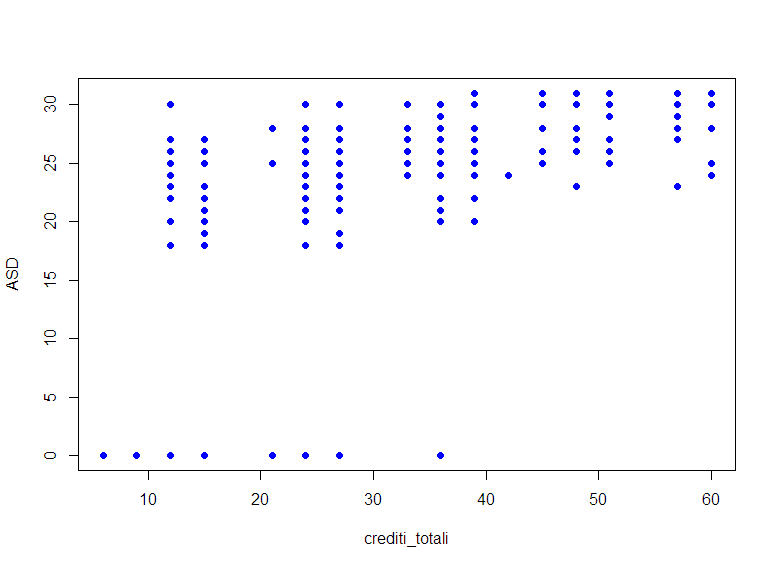
\includegraphics[width=\textwidth]{img/creditiAsd.png}
	\caption{Scatterplot tra Crediti totali e Algoritmi e strutture dati}
\end{figure}

\begin{figure}[H]
	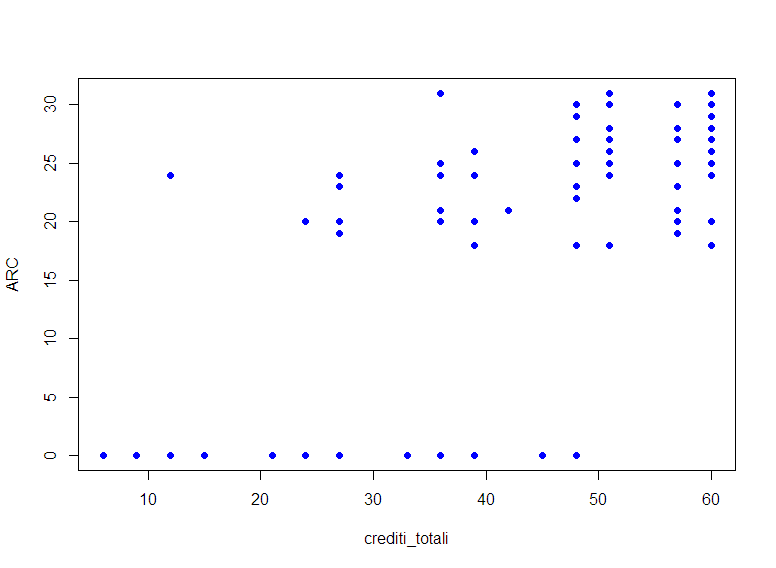
\includegraphics[width=\textwidth]{img/creditiArc.png}
	\caption{Scatterplot tra Crediti totali e Architetture degli elaboratori}
\end{figure}

L'attributo test è correlato maggiormente con l'attributo voto medio. 
Si può notare inoltre che il valore di correlazione è significativamente più alto di quello che l'attributo test ha con i voti dei singoli esami, con l'unica eccezione di MDL.
Questi valori lasciano suggerire che il punteggio conse\-guito al test d'ingresso di ogni studente sia un buon parametro per valutar\-ne l'andamento generale piuttosto che i voti di un singolo esame.
Inoltre l'attributo test mostra una discreta correlazione con i crediti totali (e quindi anche con i crediti con voto).
Per quanto riguarda le correlazioni tra i voti dei diversi esami è possibi\-le notare che il valore più alto è quello tra Architetture degli elaboratori e Programmazione che è circa pari a 0.43.
Mentre si ha una correlazione quasi nulla, ossia circa 0.10, tra il voto di Algoritmi e strutture dati e il voto di Analisi 1.

In Figura 3 sono riportati gli scatterplot tra Architetture degli elabora\-tori e Programmazione e tra Algoritmi e strutture dati  e Analisi I.
Contrariamente a quanto indicato dai valori delle correlazioni tra le due coppie di attributi, 
gli scatterplot mostrati in Figura 3, sembrano suggerire una correlazione simile (se non migliore) tra Algoritmi e Strutture dati e Analisi 1, rispetto a quella tra Architetture e Programmazione.
Questo fenomeno è dovuto al fatto che un notevole numero di studenti non ha sostenuto ne architteture ne programmazione. 
Tuttavia, in uno scatterplot non è possibile distinguere oggetti con gli stessi valori per gli attributi considerati e quindi i dati che influenzano maggiormente la correlazione tra Architetture e Programmazione non vengono essenzialmente mostrati (rappresentati tramite singolo punto) nel grafico in questione.  
D'altra parte, gli studenti che non hanno sostenuto ne Algoritmi ne Analisi 1 sono molti meno e quindi influenzano in mondo meno significativo la correlazione tra tali attributi. 
In Figura 4 sono mostrati gli scatterplot realizzati con Weka applicando piccole variazioni casuali ai punti per distinguere i dati che hanno valori identici (Jitter). 
Utilizzando questa tecnica è quindi possibile notare i seguenti fatti:
\begin{enumerate}
	\item Il numero di studenti che non ha sostenuto ne Architteture ne Program\-mazione è, come abbiamo già detto, notevolmente superiore al numero di studenti che non hanno sostenuto ne algoritmi ne analisi 1. La presenza di studenti con queste caratteristiche influenza quindi mag\-giormente la correlazione complessiva tra Architetture e Programma\-zione rispetto a quella tra Algoritmi e Analisi1; 
	\item Gli studenti che hanno sostenuto Programmazione ma non hanno sostenuto Architetture sono molti di più rispetto a quelli che hanno sostenuto Analisi 1 ma non hanno sostenuto Algoritmi. Viceversa, gli studenti che hanno sostenuto Architetture ma non Programmazione sono molti meno di quelli che hanno sostenuto Algoritmi ma non Analisi 1. Gli studenti con queste caratteristiche (110 per Architetture e Programma\-zione, 127 per Algoritmi e Analisi1) non evidenziano correlazioni tra le due diverse coppie di attributi ed essendo in quantità paragonabili influenzeranno le correlazione complessive tra le due diverse coppie di attributi circa in egual misura;
	\item Confrontando gli studenti che hanno sostenuto sia Architetture che Pro\-grammazione con quelli che hanno sostenuto sia Algoritmi che Analisi 1 si nota una migliore correlazione per la seconda coppia di attributi su tali sottoinsiemi del dataset. Tuttavia, essendo i due sottoinsieme (studenti che hanno sostenuto sia Architetture che Pro\-gramma\-zione e studenti che hanno sostenuto sia Algoritmi che Analisi 1) di dimensioni paragonabili influenzeranno in modo minore la correlazione complessiva rispetto a quanto lo fanno gli oggetti discussi al punto 1.
\end{enumerate}
Per dimostrare la tesi secondo cui gli studenti che non hanno sostenuto ne Architetture ne Programmazione influenzano in modo decisivo la correlazione tra questi due attributi è possibile calcolare la correlazione tra i due attributi sul sottoinsieme del dataset privo di questi oggetti. 
In questo caso infatti la correlazione tra i due attributi è T. 
Se eseguiamo la stessa operazione rispetto però agli attributi Algoritmi e Analisi 1 otteniamo una correlazione pari a Z. 
La differenza tra le correlazioni delle due diverse coppie di attributi è minore.

\begin{figure}[H]
	\centering
	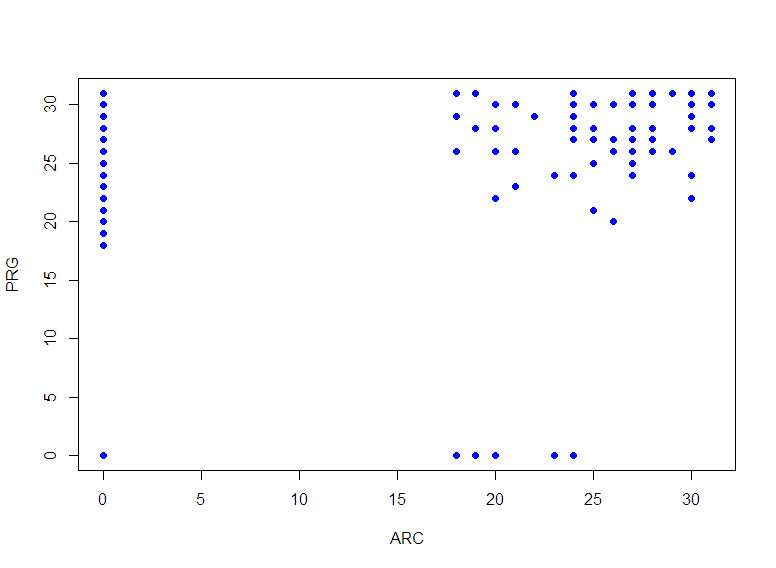
\includegraphics[width=\textwidth, height=21em]{img/arcPrg.png}
	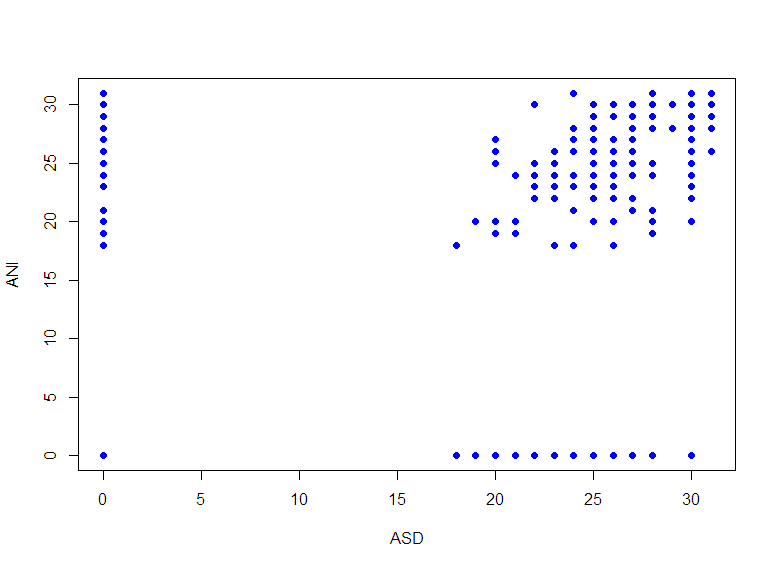
\includegraphics[width=\textwidth, height=21em]{img/asdAni.png}
	\caption{Scatterplot tra Architetture degli elaboratori e Programmazione e tra Algoritmi e strutture dati e Analisi I}
\end{figure}

\begin{figure}[H]
	\centering
	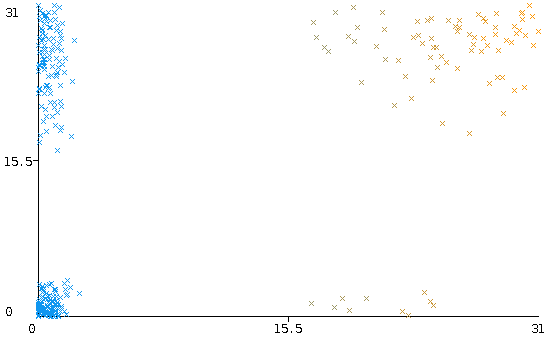
\includegraphics[width=\textwidth]{img/arcPrgWeka.png}
	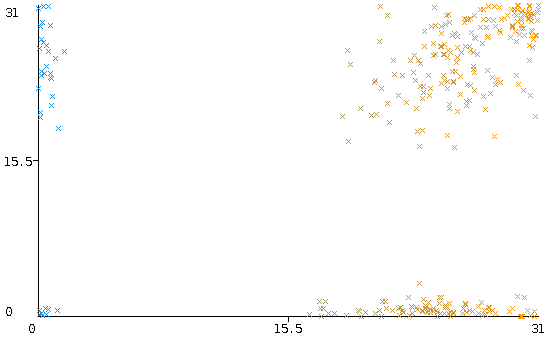
\includegraphics[width=\textwidth]{img/asdAniWeka.png}
	\caption{Scatterplot tra Architetture degli elaboratori e Programmazione e tra Algoritmi e strutture dati e Analisi I con Jitter}
\end{figure}

\begin{figure}[H]
	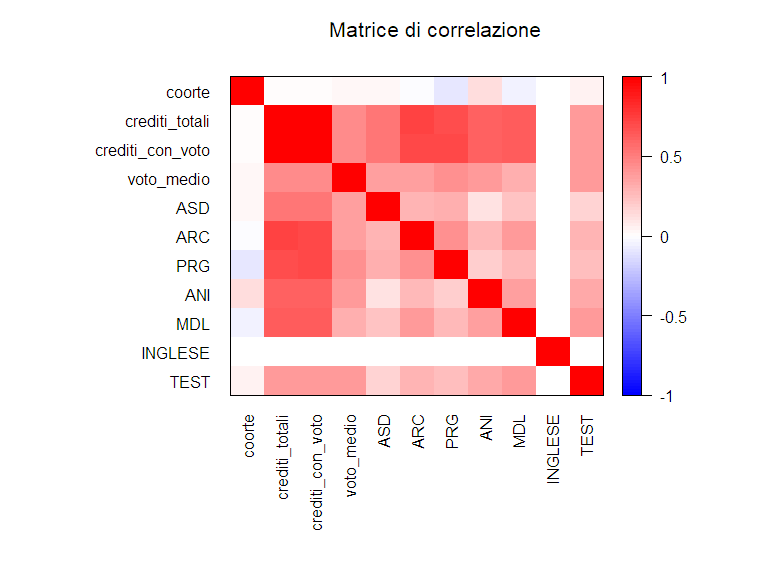
\includegraphics[width=\textwidth]{img/corMatrix.png}
	\caption{Matrice di correlazione}
	\label{fig:cMatrix}
\end{figure}

In Figura~\ref{fig:cMatrix} viene riportata la matrice di correlazione.
Per applicare gli algoritmi di clustering è stato utilizzato il software Weka. Tuttavia prima di applicare tali algoritmi è stato necessaria un ulteriore fase di preprocessing
nella quale sono stati normalizzati tutti gli attributi del data\-set in una scala di valori compresi tra zero e uno in modo da evitare problemi dovuti alle diverse scale di valori degli attributi.

\newpage
\section{Clustering}
\label{cap:clust}
In questo capitolo verranno effettuate alcune analisi di clustering sui se\-guenti attributi:
\begin{itemize}
\item crediti totali, architetture, programmazione;
\item algoritmi e strutture dati, architetture, programmazione, analisi 1 e matematica discreta e logica;
\item voto medio e test.
\end{itemize}
Le tecniche di clustering utilizzate sono il clustering gerarchico, l'algori\-tmo di Kmeans e infine l'algoritmo DBSCAN. In particolare:
\begin{itemize}
\item l'analisi effettuata con tecniche di clustering gerarchico è stata effet\-tuata su un sottoinsieme dei dati a disposizione selezionato in base alla coorte dello studente (anno 2010);
\item nel caso dell'algoritmo di Kmeans viene stabilito preventivamente il numero dei cluster possibili utilizzando valori ritenuti sensati di volta in volta;
\item l'algoritmo DBSCAN è stato utilizzato per l'analisi relativa ai voti dei diversi esami scegliendo preventivamente i valori di \texttt{MinPts} e \texttt{eps} ritenuti sensati di volta in volta.
\end{itemize}
Fatta eccezione per l'algoritmo DBSCAN tutte le analisi condotte sono state effettuate dopo la normalizzazione degli attributi coinvolti. 
Per la valutazione dei risultati ottenuti si rimanda al capitolo \ref{cap:val-clust} dove viene ana\-liz\-zata la validità dei risultati ottenuti e sono determinati: 
numero di cluster ottimali per l'algoritmo di Kmeans e valo\-re di \texttt{eps} ottimale per DBSCAN.
Come prima analisi viene mostrata quella relativa ai tre attributi del data\-set maggiormente correlati (a meno di 
correlazioni ovvie) ossia crediti totali, architetture e programmazione.
È stato utilizzato l'algoritmo di Kmeans implementato in Weka specificando ini\-zialmente un numero di cluster pari a due, lasciando i valori di default per la generazione dei centroidi.
In Tabella \ref{c2AP} sono riporta\-te le coordinate dei centroidi relativi all'esecuzione dell'algoritmo con un valore di k pari a 2.
% Cluster# 2 sse 51.35
% Attribute         Full Data          0          1
%                     (316.0)    (183.0)    (133.0)
% =================================================
% crediti_totali        0.496     0.6542     0.2782
% ARC                  0.2126     0.3295     0.0519
% PRG                  0.4929      0.851          0
% Clustered Instances
% 0      183 ( 58%)
% 1      133 ( 42%)
\begin{table}[ht]
	\centering
	\begin{tabular}{@{}lllll@{}}
	\toprule
	  & Crediti totali & ARC  & PRG  & Istanze\\ \midrule
	0 & 0.65           & 0.32 & 0.85 & 183 ( 58\%)\\
	1 & 0.27           & 0.05 & 0    & 133 ( 42\%)\\ \bottomrule
	\end{tabular}
	\caption{Cluster con ARC e PRG con k = 2 SSE 51.35}
	\label{c2AP}
\end{table}
Come si può notare dalle coordinate dei centroidi questa prima esecuzione dell'algoritmo suddivide il dataset in due gruppi piuttosto distinti.
Il valore della somma degli errori al quadrato (SSE) in questa esecuzione è risultata pari a 51.35.
In Tabella \ref{c3AP} sono riportate le coordinate dei centroidi relativi all'esecuzione dell'algoritmo con un valore di k pari a 3.
% Cluster# 3 sse 14.85
% Attribute         Full Data          0          1          2
%                     (316.0)     (73.0)    (133.0)    (110.0)
% ============================================================
% crediti_totali        0.496      0.882     0.2782      0.503
% ARC                  0.2126     0.8259     0.0519          0
% PRG                  0.4929     0.8979          0     0.8199
% Clustered Instances
% 0       73 ( 23%)
% 1      133 ( 42%)
% 2      110 ( 35%)
\begin{table}[ht]
	\centering
	\begin{tabular}{@{}lllll@{}}
	\toprule
	  & Crediti totali & ARC  & PRG  & Istanze\\ \midrule
	0 & 0.88           & 0.82 & 0.89 & 73 ( 23\%)\\
	1 & 0.27           & 0.05 & 0    & 133 ( 42\%)\\
	2 & 0.50           & 0    & 0.81 & 110 ( 35\%)\\ \bottomrule
	\end{tabular}
	\caption{Cluster con ARC e PRG con k = 3 SSE 14.85}
	\label{c3AP}
\end{table}
In questo caso il valore di SSE è pari a 14.85. È inoltre possibile constatare come l'algoritmo di K-means abbia messo in evidenza tre tipologie ben distinte di studenti:
\begin{itemize}
	\item Gli studenti appartenenti al cluster 0 sono gli studenti "migliori" a\-vendo sostenuto la quasi totalità degli esami del primo anno alla fine della sessione estiva e riportando delle ottime valutazioni per quanto riguarda gli esami di Architetture e di Programmazione;
	\item La seconda categoria di studenti (cluster 1) sono gli studenti "peg\-giori" che hanno sostenuto pochi esami e nel caso specifico delle materie considerate hanno conseguito valutazioni basse o non hanno sostenuto l'esame;
	\item Infine gli studenti appartenenti all'ultimo cluster sono gli studenti che hanno sostenuto Programmazione con un buon voto ma non hanno fatto l'esame di Architetture.
\end{itemize}
Come si evince analizzando i tre cluster in particolare notando le diverse combinazioni dei valori assunti dai centroidi dei voti, si capisce come sia assente la categoria di studenti che ha sostenuto con profitto l'esame di architetture, ma non ha sostenuto l'esame di programmazione,
lasciando quindi intendere che se uno studente ha sostenuto l'esame di architetture allora generalmente ha sostenuto con una buona valutazione l'esame di programmazione.

In Figura \ref{fig:dendo-complete} è mostrato il dendogramma relativo al clustering gerarchico con metodo complete mentre in Figura \ref{fig:dendo-average} viene mostrato il dendogramma relativo al clustering gerarchico con metodo average per questa prima analisi.
\begin{figure}[H]
	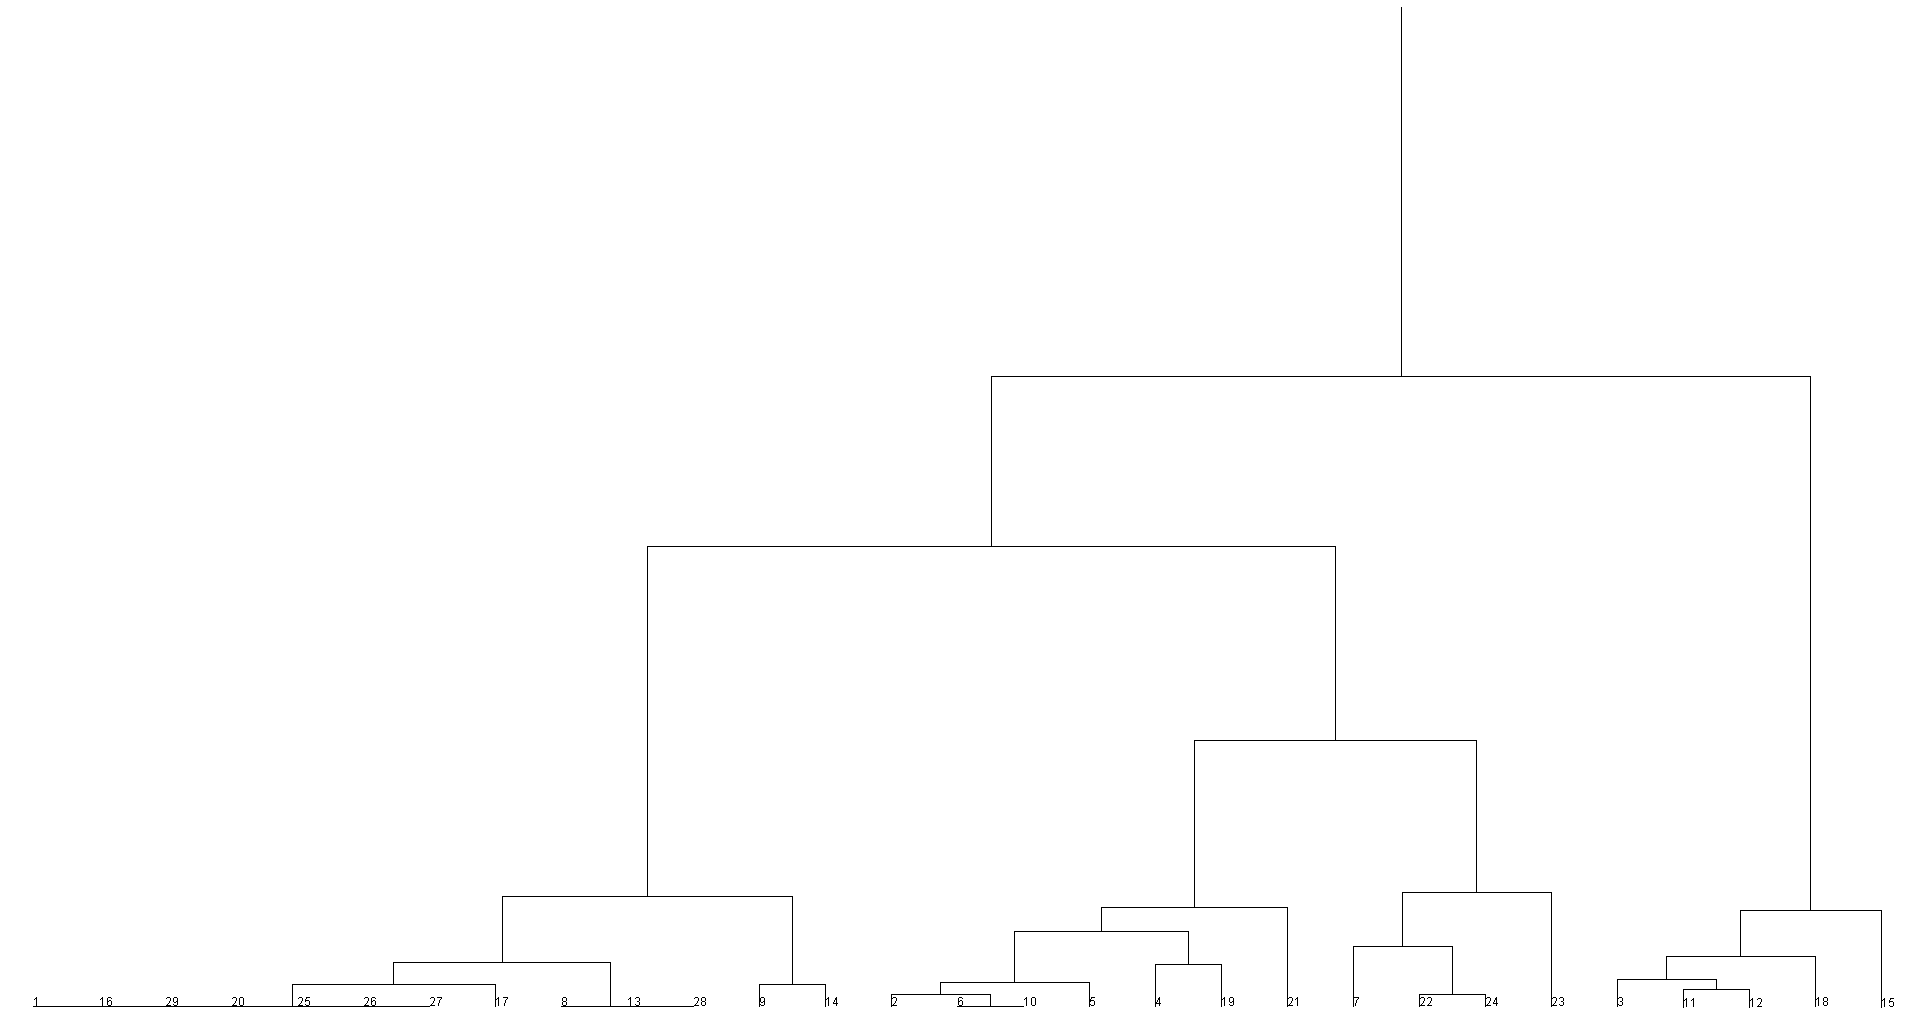
\includegraphics[width=\textwidth]{img/hierarchical-complete.png}
	\caption{Dendogramma relativo al clustering gerarchico con metodo complete.}
	\label{fig:dendo-complete}
\end{figure}
\begin{figure}[H]
	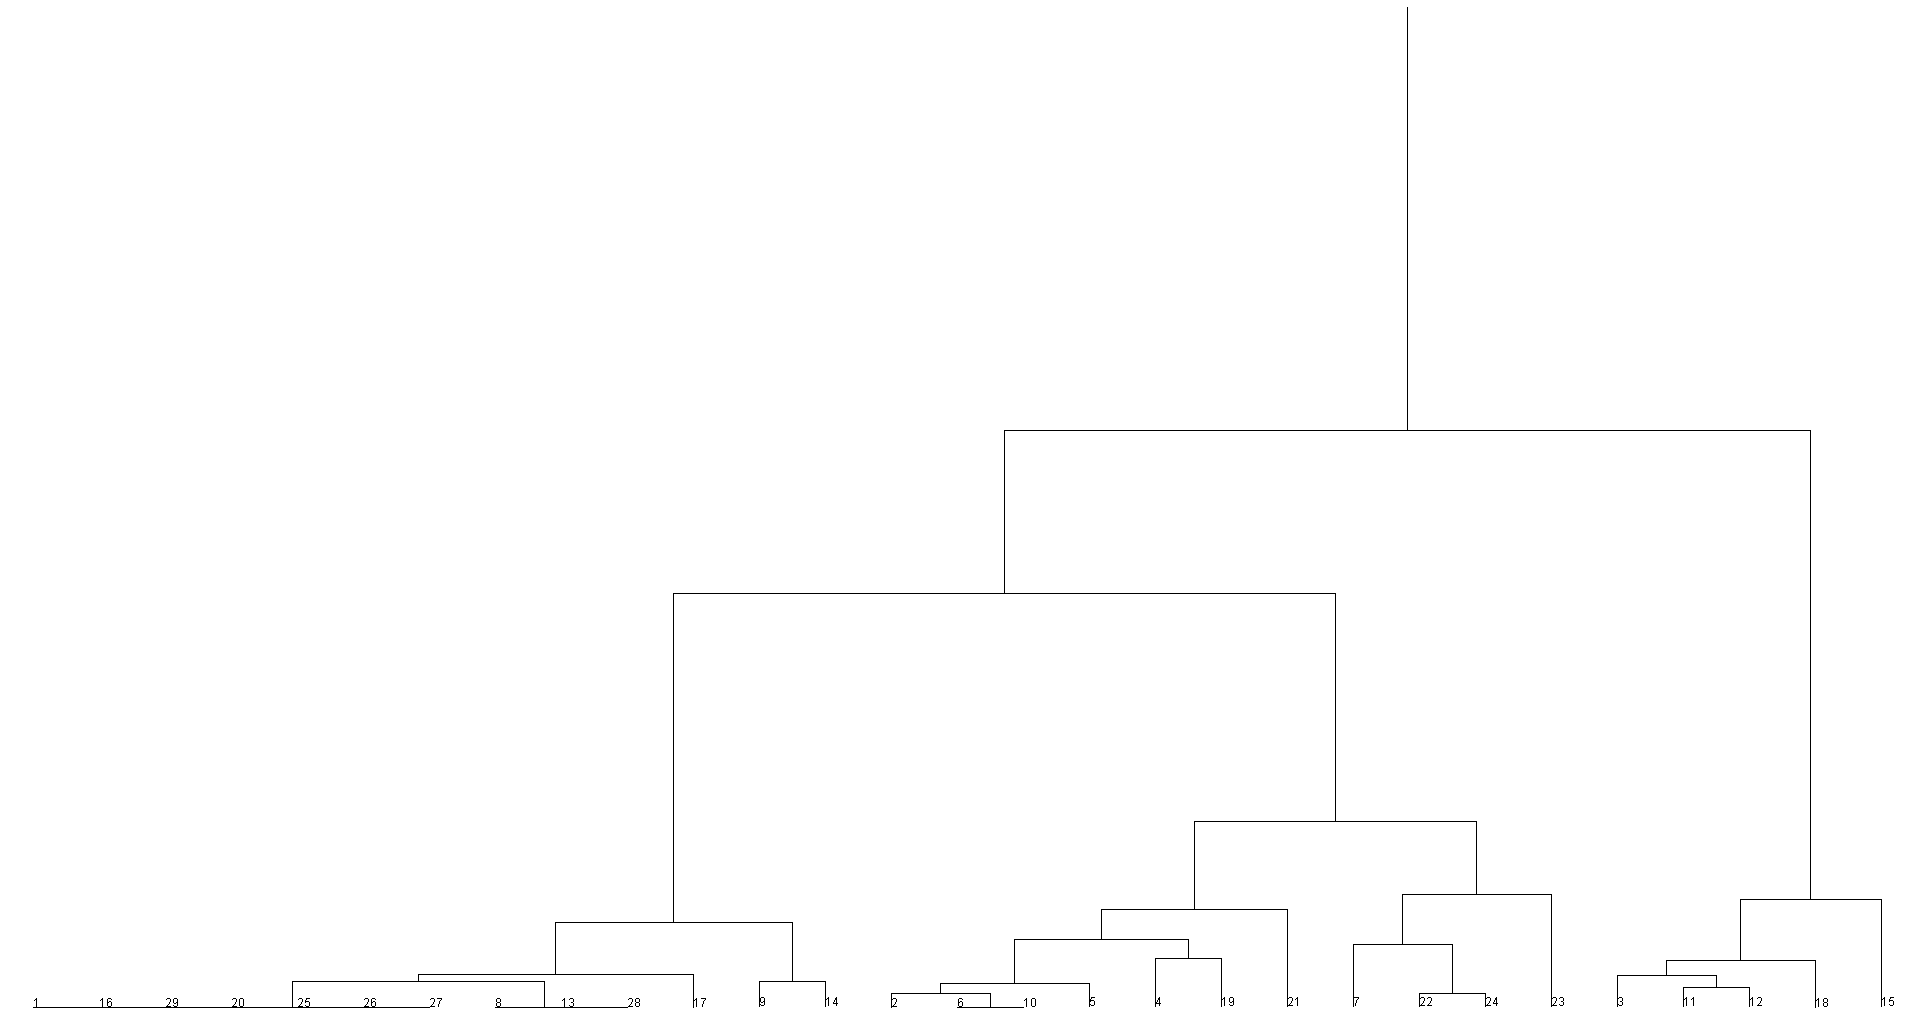
\includegraphics[width=\textwidth]{img/hierarchical-average.png}
	\caption{Dendogramma relativo al clustering gerarchico con metodo average.}
	\label{fig:dendo-average}
\end{figure}
% Cluster# 2 sse 12.4
% Attribute     Full Data          0          1
%                 (316.0)    (134.0)    (182.0)
% =============================================
% voto_medio       0.5684     0.3823     0.7054
% TEST             0.5996     0.4958      0.676
% Clustered Instances

% 0      134 ( 42%)
% 1      182 ( 58%)
% \begin{table}[ht]
% 	\centering
% 	\caption{Cluster con Voto\_medio e Test con k = 2 SSE 12.4}
% 	\label{c2MT}
% 	\begin{tabular}{@{}lllll@{}}
% 	\toprule
% 	  & voto medio & Test  & Istanze\\ \midrule
% 	0 & 0.38       & 0.49  & 134 ( 42\%)\\
% 	1 & 0.70       & 0.67  & 182 ( 58\%)\\ \bottomrule
% 	\end{tabular}
% \end{table}

La seconda analisi che è stata condotta è quella relativa ai voti conse\-guiti dagli studenti del primo anno durante la sessione estiva. In questo caso l'algoritmo di K-means è stato inizializzato con un valore di $k=3$.
In Tabella \ref{c3V} sono riportate le coordinate dei centroidi al termine dell'algori\-tmo. 
% Attribute    Full Data          0          1          2
%                (316.0)    (100.0)    (133.0)     (83.0)
% =======================================================
% ASD             0.7502      0.739     0.6551     0.9161
% ARC             0.2126     0.0565     0.0519     0.6584
% PRG             0.4929     0.8168          0     0.8923
% ANI             0.5787     0.4303     0.5006     0.8826
% MDL             0.2169     0.0223     0.1208     0.6055
% 0      100 ( 32%)
% 1      133 ( 42%)
% 2       83 ( 26%) SSE106.19
\begin{table}[ht]
	\centering
	\begin{tabular}{@{}lllllll@{}}
	\toprule
	  & ASD  & ARC  & PRG & ANI  & MDL  & Istanze      \\ \midrule
	0 & 0.73 & 0.05 & 0.81& 0.43 & 0.02 &  100  ( 32\%)\\
	1 & 0.65 & 0.05 & 0   & 0.50 & 0.12 &  133 ( 42\%) \\
	2 & 0.91 & 0.65 & 0.89& 0.88 & 0.60 &  83  ( 26\%) \\ \bottomrule
	\end{tabular}
	\caption{Cluster di tutti i voti con k = 3 SSE 106.19}
	\label{c3V}
\end{table}
In questo caso sono quindi stati determinati i profili di tre diversi gruppi di studenti:
\begin{itemize}
\item gli studenti che hanno conseguito una buona votazione negli esami di Algoritmi e Strutture Dati e Programmazione,
una votazione dis\-creta all'esame di Analisi I e che non hanno sostenuto Matematica discreta e Logica e Architetture degli elaboratori (Cluster 0);
\item gli studenti con le stesse caratteristiche del cluster precedente, ma che non hanno sostenuto Programmazione (Cluster 1);
\item gli studenti che hanno sostenuto tutti gli esami e con un buona vota\-zione (Cluster 2).
\end{itemize}
In Figura \ref{APC} è riportato lo scatter plot relativo ai voti di Architetture degli Elaboratori e Programmazione che sono
maggiormente correlati. Il valore di SSE in questo caso è pari a 106.19. 
Come è stato specificato all'inizio del capitolo, in questo caso è stato utilizzato anche l'algoritmo DBSCAN per effettuare il clustering degli attributi scelti. 
Inoltre, poiché gli attributi scelti per l'analisi in questo caso hanno valori nello stesso intervallo $[0,31]$ non è stato necessario procedere alla normalizzazione. 
Quindi, analoga\-mente a quanto fatto con l'algoritmo di K-means, i parametri con cui ese\-guire l'algoritmo sono stati scelti basandosi sull'intuizione e sulla cono\-scenza del problema. 
Per la valutazione dei risultati ottenuti e la scelta del valore ottimale di \texttt{eps} in funzione di \texttt{MinPts} si rimanda al capitolo \ref{cap:val-clust}. 

In Tabella \ref{tab:dbscan605} sono riportati i cluster ottenuti e la proporzione di istanze al loro interno eseguendo l'algoritmo DBSCAN con \texttt{MinPts=6} e \texttt{eps=0.5}. 
In questo caso $38$ record dei $316$ totali sono stati marcati come rumore dall'algoritmo.
Inoltre, è possibile notare che alcuni dei cluster prodotti hanno delle dimensioni decisamente ridotte. Infatti, il cluster 6 contiene solo 6 record dei 316 totali, mentre il cluster 3, il cluster 7 e il cluster 9 contengono solo, rispettivamente 13, 18 e 14 record.
Il cluster 8 sembra rappresentare un caso limite con 22 record complessivi.
In ogni caso, un numero così elevato di cluster di dimensioni ridotte sembra suggerire che il valore di \texttt{MinPts} sia troppo basso e che i gruppi di oggetti riconosciuti come cluster  che hanno dimensione ridotta siano in realtà gruppi di outliers.
In Tabella \ref{tab:dbscan1004} sono riportati i medesimi risultati eseguendo l'algoritmo DBSCAN con \texttt{MinPts=10} e \texttt{eps=0.4}. 
In questo caso, i risultati ottenuti sembrano confermare le nostre aspettative poiché i record marcati come rumore dall'algoritmo diventano $44$.
Inoltre, il numero di cluster determinati dall'algoritmo è diminuito di uno e i cluster di dimensioni significativamente ridotte sono solamente il cluster 3 e il cluster 8.
L'esecuzione dell'algoritmo con un numero maggiore di \texttt{MinPts} sembrerebbe quindi produrre un clustering migliore.
Andando a incrementare ulteriormente il valore di \texttt{MinPts} ponendo \texttt{MinPts} a 20 si ottiene il clustering mostrato in Tabella \ref{tab:dbscan2004}.
In questo caso, il numero di cluster scende ulteriormente di tre e inoltre la distribuzione dei record nei cluster risulta decisamente più uniforme e non sono presenti dei cluster di dimensioni significativamente piccole.
Inoltre, in questo caso 89 dei 316 record totali sono stati marcati come rumore dall'algoritmo.

In Figura \ref{fig:dendo-complete2} è mostrato il dendogramma relativo al clustering gerarchico con metodo complete mentre in Figura \ref{fig:dendo-average2} viene mostrato il dendogramma relativo al clustering gerarchico con metodo average per la seconda analisi. 
\begin{figure}[H]
	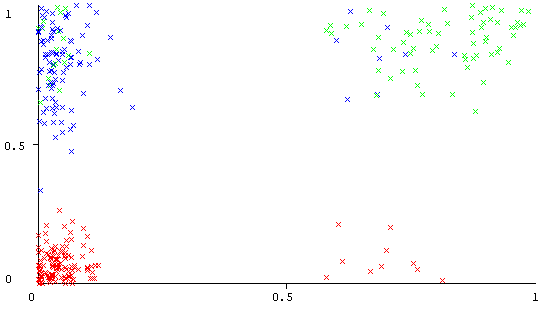
\includegraphics[width=\textwidth]{img/ARC-PRG-Cluster.png}
	\captionsetup{justification=centering}
	\caption{Scatter plot relativo ai cluster dei voti di Architetture degli Elaboratori e Programmazione}
	\label{APC}
\end{figure}
\begin{table}[H]
\centering
\begin{tabular}{@{}ll@{}}
\toprule
                        & Istanze  \\\midrule
\multicolumn{1}{l}{0} & 40 (14\%)  \\
\multicolumn{1}{l}{1} & 46 (17\%)  \\
\multicolumn{1}{l}{2} & 41 (15\%)  \\
\multicolumn{1}{l}{3} & 13 (5\%)   \\
\multicolumn{1}{l}{4} & 45 (16\%)  \\
\multicolumn{1}{l}{5} & 33 (12\%)  \\
\multicolumn{1}{l}{6} & 6  (2\%)   \\
\multicolumn{1}{l}{7} & 18 (6\%)   \\
\multicolumn{1}{l}{8} & 22 (8\%)   \\
\multicolumn{1}{l}{9} & 14 (5\%)   \\\bottomrule
\end{tabular}
\caption{Cluster ottenuti con DBSCAN eseguito con \texttt{MinPts=6} e \texttt{eps=0.5}. Molti dei cluster prodotti hanno dimensioni notevolmente ridotte.}
\label{tab:dbscan605}
\end{table}
\begin{table}[H]
\centering
\begin{tabular}{@{}ll@{}}
\toprule
                        & Istanze    \\ \midrule
\multicolumn{1}{l}{0}   & 40 (15\%)  \\ 
\multicolumn{1}{l}{1}   & 46 (17\%)  \\ 
\multicolumn{1}{l}{2}   & 41 (15\%)  \\ 
\multicolumn{1}{l}{3}   & 13 (5\%)   \\ 
\multicolumn{1}{l}{4}   & 45 (17\%)  \\ 
\multicolumn{1}{l}{5}   & 33 (12\%)  \\ 
\multicolumn{1}{l}{6}   & 18 (7\%)   \\ 
\multicolumn{1}{l}{7}   & 22 (8\%)   \\ 
\multicolumn{1}{l}{8}   & 14 (5\%)   \\ \bottomrule
\end{tabular}
\caption{Cluster ottenuti con DBSCAN eseguito con \texttt{MinPts=10} e \texttt{eps=0.4}. In questo caso di ottengono meno cluster e si riduce il numero di cluster di dimensioni ridotte.}
\label{tab:dbscan1004}
\end{table}
\begin{table}[H]
\centering
\begin{tabular}{@{}ll@{}}
\toprule
                        & Istanze  \\ \midrule
\multicolumn{1}{l}{0} & 40 (18\%) \\
\multicolumn{1}{l}{1} & 46 (20\%) \\
\multicolumn{1}{l}{2} & 41 (18\%) \\
\multicolumn{1}{l}{3} & 45 (20\%) \\
\multicolumn{1}{l}{4} & 33 (15\%) \\
\multicolumn{1}{l}{5} & 22 (10\%) \\ \bottomrule
\end{tabular}
\caption{Cluster ottenuti con DBSCAN eseguito con \texttt{MinPts=20} e \texttt{eps=0.4}. In questo caso la distribuzione dei record nei cluster risulta decisamente più uniforme.}
\label{tab:dbscan2004}
\end{table}
\begin{figure}[H]
	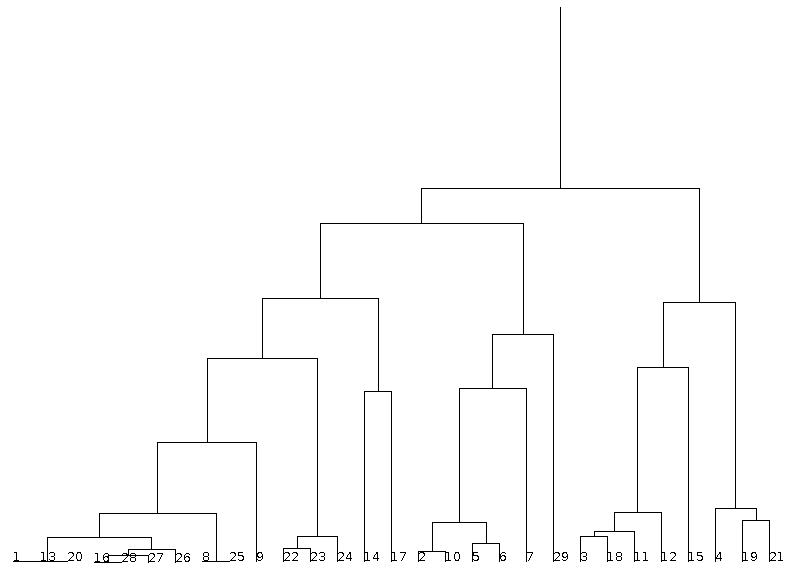
\includegraphics[width=\textwidth]{img/c-gerarchico-voti-complete.png}
	\caption{Dendogramma relativo al clustering gerarchico con metodo complete.}
	\label{fig:dendo-complete2}
\end{figure}
\begin{figure}[H]
	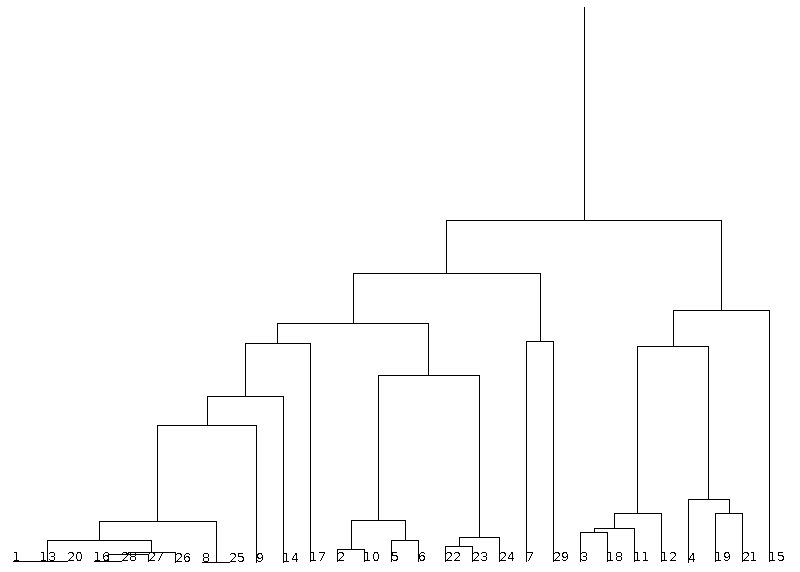
\includegraphics[width=\textwidth]{img/c-gerarchico-voti-average.png}
	\caption{Dendogramma relativo al clustering gerarchico con metodo average.}
	\label{fig:dendo-average2}
\end{figure}

Infine, l'ultima analisi che è stata condotta riguarda gli attributi test e voto medio. È stato scelto di analizzare 
questi due attributi congiuntamen\-te in quanto, come è stato detto nel capitolo precedente, l'attributo voto medio 
presenta una buona correlazione con l'attributo test. 
In Tabella \ref{c3MT} sono riportate le coordinate dei centroidi relativi all'esecuzione dell'algori\-tmo con un numero di cluster pari a 3.
% Cluster# 3 sse 9.6
% Attribute     Full Data          0          1          2
%                 (316.0)     (85.0)    (146.0)     (85.0)
% ========================================================
% voto_medio       0.5684     0.3665     0.7529     0.4534
% TEST             0.5996     0.4188     0.6622     0.6729
% Clustered Instances
% 0       85 ( 27%)
% 1      146 ( 46%)
% 2       85 ( 27%)
\begin{table}[ht]
	\centering
	\begin{tabular}{@{}llll@{}}
	\toprule
	  & voto medio & Test  & Istanze\\ \midrule
	0 & 0.36       & 0.41  & 85  ( 27\%)\\
	1 & 0.75       & 0.66  & 146 ( 42\%)\\
	2 & 0.45       & 0.67  & 85  ( 27\%)\\ \bottomrule
	\end{tabular}
	\caption{Cluster con Voto\_medio e Test con k = 3 SSE 9.6}
	\label{c3MT}
\end{table}
In questo caso è possibile notare come
l'algoritmo di K-means determini tre cluster ben definiti che suddi\-vidono il dataset tra gli studenti che hanno una
media complessiva mag\-giore e un voto al test d'ingresso alto e quelli che invece hanno una media più bassa e 
hanno conseguito punteggio basso al test di ingresso. Questi gruppi determinati sono coerenti con la correlazione 
che esiste tra i due attributi che tuttavia non è particolarmente elevata (diversamente dagli attributi presi in 
considerazione nell'analisi precedente). Infatti, oltre ai primi due cluster che identificano gli studenti "migliori"
e quelli "peggiori" esiste un terzo cluster di studenti che hanno conseguito un punteggio al test d'ingresso decisamente
positivo, ma non hanno mantenuto una media dei voti altrettanto buona. Il valore del SSE in questo caso è 9.6. 

In Figura \ref{fig:dendo-complete3} è mostrato il dendogramma relativo al clustering gerar\-chico con metodo complete mentre in Figura \ref{fig:dendo-average3} viene mostrato il dendo\-gramma relativo al clustering gerarchico con metodo average per la terza e ultima analisi condotta.
\begin{figure}[H]
	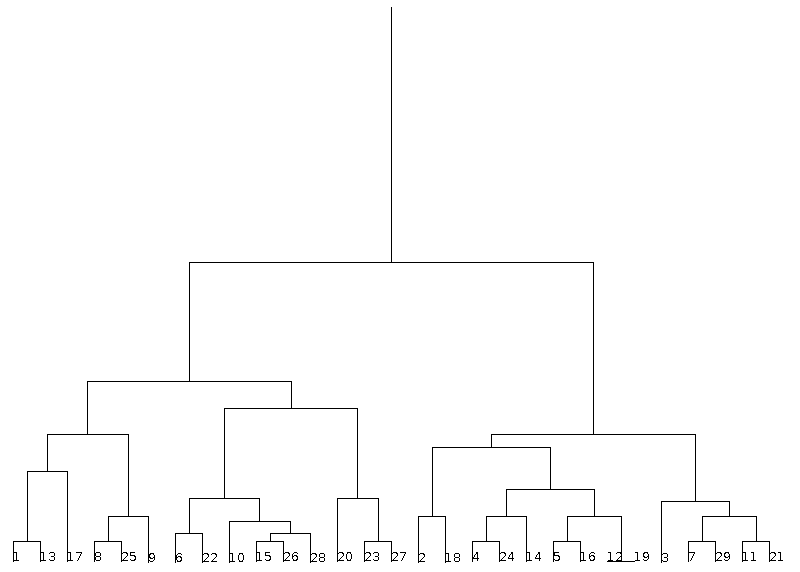
\includegraphics[width=\textwidth]{img/c-gerarchico-vmedio-test-complete.png}
	\caption{Dendogramma relativo al clustering gerarchico con metodo complete.}
	\label{fig:dendo-complete3}
\end{figure}
\begin{figure}[H]
	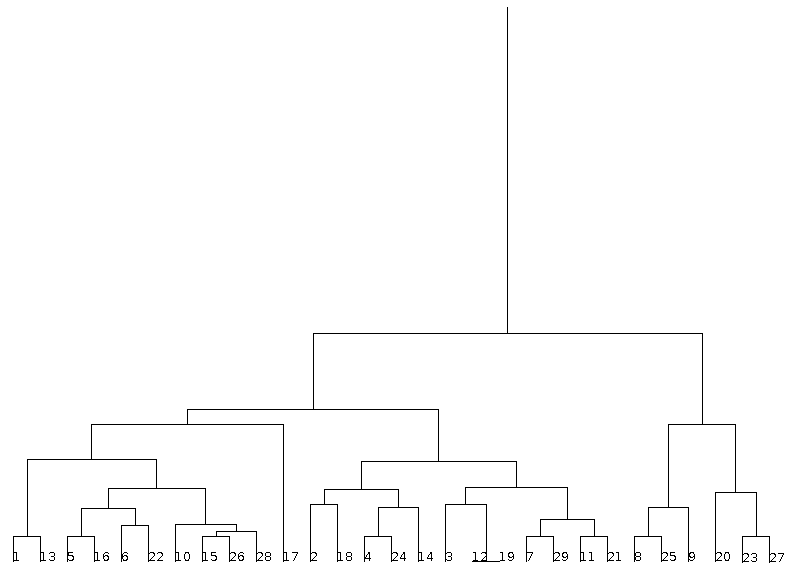
\includegraphics[width=\textwidth]{img/c-gerarchico-vmedio-test-average.png}
	\caption{Dendogramma relativo al clustering gerarchico con metodo average.}
	\label{fig:dendo-average3}
\end{figure}
\newpage
\section{Valutazione del clustering e model selection}
\label{cap:val-clust}
In questo capitolo vengono presi in considerazione alcuni metodi per scegliere i parametri con cui inizializzare gli algoritmi di K-means e DBSCAN e vengono analizzati i risultati ottenuti nel capitolo \ref{cap:clust}.
Nel capitolo prece\-dente, infatti, l'algoritmo di K-means è stato eseguito scegliendo preventi\-vamente il numero di cluster possibili (tipicamente 2 o 3) basandosi esclu\-sivamente sull'intuizione e quindi senza avere garanzie circa la bontà e corret\-tezza dei risultati ottenuti. 
In questo capitolo viene valutata la vali\-dità delle analisi di clustering effettuate con l'algoritmo K-means e viene utilizzata una procedura basata sul SSE che tenta di determinare il valore ottimale di $k$ con cui inizializzare l'algoritmo di K-means in modo da mi\-gliorarne la validità. 

Per ciascuno degli aspetti analizzati vengono quindi eseguite le seguenti operazioni:

\begin{enumerate}
\item determinazione dei valori del SSE in funzione di $k$;
\item \label{item:k-opt} scelta di $k_{opt}$ come il più piccolo $k$ per cui il valore del SSE "smette di decrescere";
\item \label{item:corr-neg} confronto del valore di correlazione ottenuta tra la matrice di incidenza e quella delle distanze per i valori di $k=2$, $k=3$ e $k_{opt}$.
\end{enumerate}
Per quanto riguarda il Punto \ref{item:k-opt} è necessario approssimare il valore di $k_{opt}$ scegliendo, ad esempio, il primo valore di $k$ per cui si verifica una varia\-zione nel SSE minore di una quantità fissata $\varepsilon$. 
Per quanto concerne il Punto \ref{item:corr-neg} si ha che un valore inferiore della correlazione (sperabilmente negativo) indica un miglior risultato di clustering poiché, idealmente, punti appartenenti allo stesso cluster (quindi con valore di incidenza $1$) dovreb\-bero trovarsi a una distanza minore. Quindi, per i tre attributi crediti totali, architetture e programmazione su cui è stata fatta la prima analisi con l'algoritmo di K-means si ottiene il grafico $k-SSE$ riportato in Figura \ref{fig:k-sse1}.

\begin{figure}[H]
	\centering
	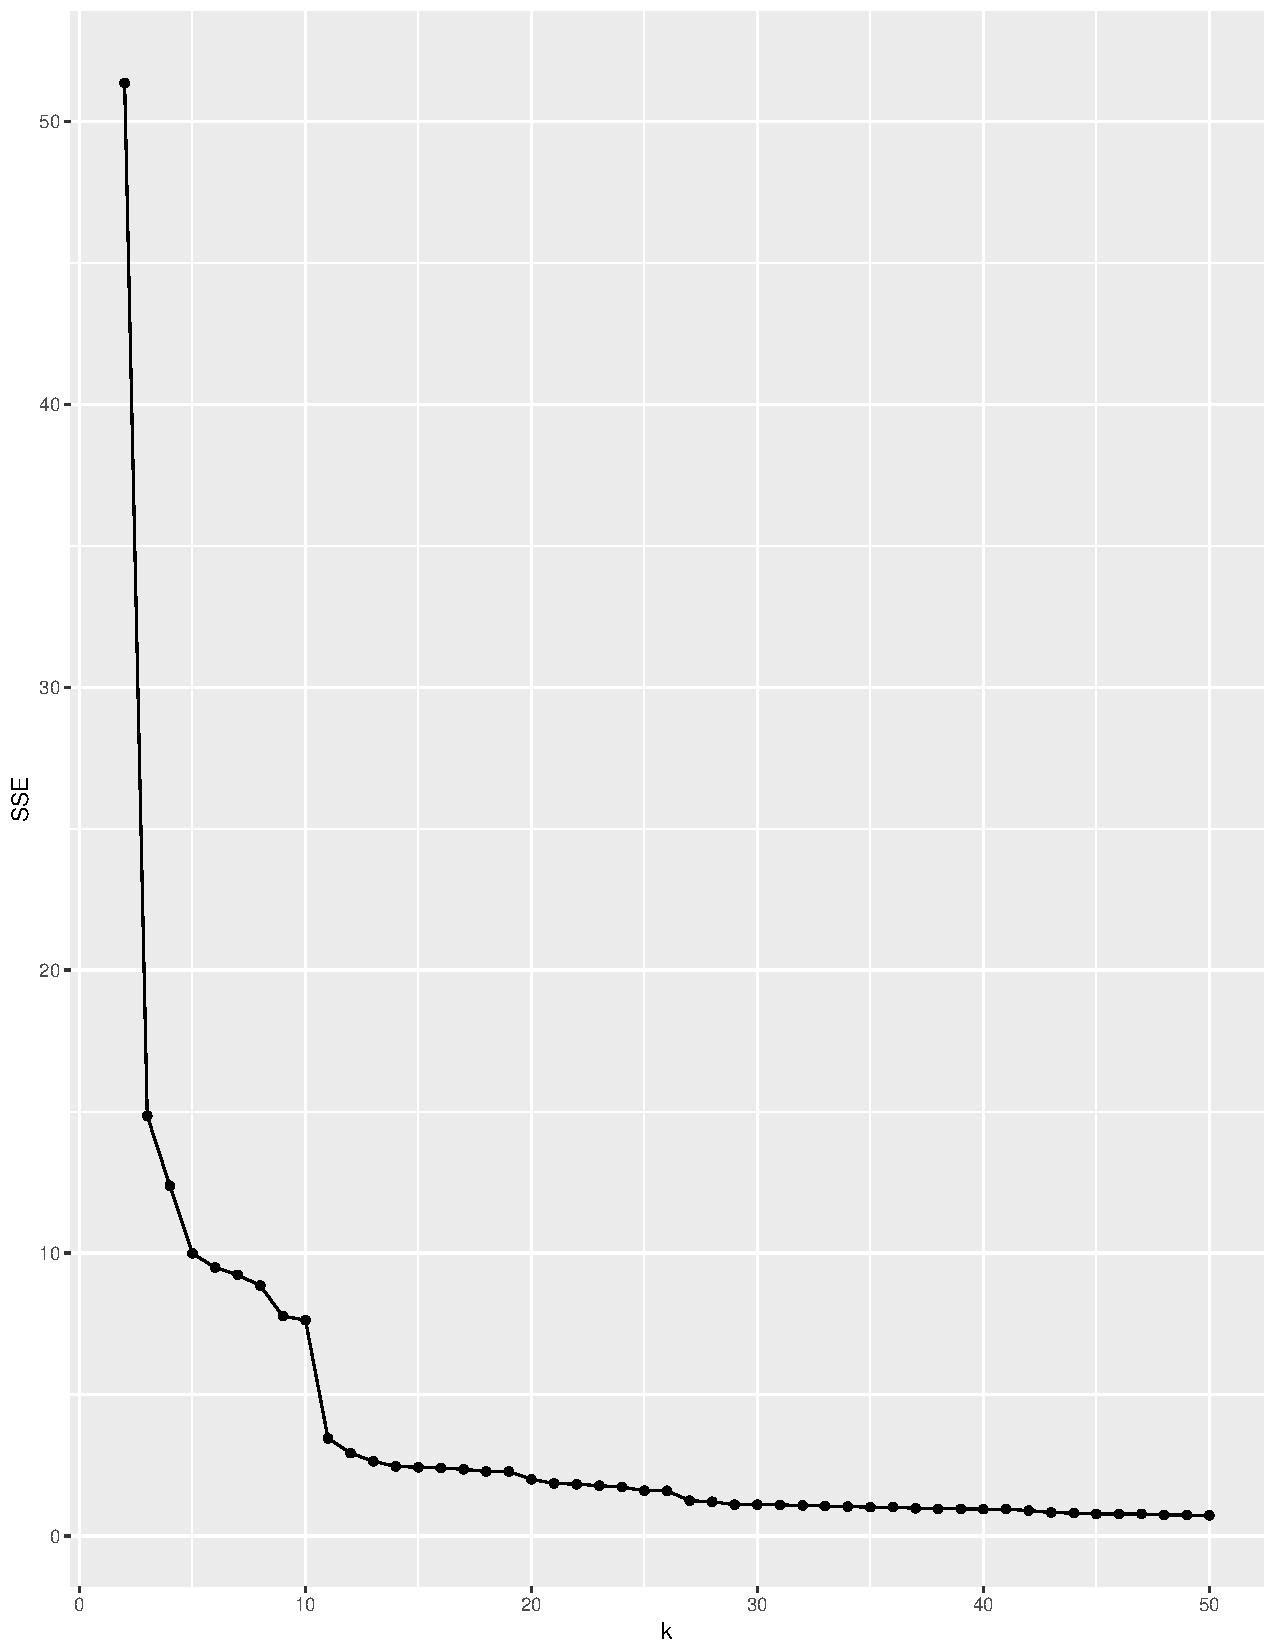
\includegraphics[width=\textwidth, height=12cm,keepaspectratio]{img/k-sse-crediti-totali-arc-prg.pdf}
	\caption{Andamento del valore del $SSE$ in funzione del valore di $k$.}
	\label{fig:k-sse1}
\end{figure}

Scegliendo il valore minimo di $\varepsilon=0.01$ (dato che è stato scelto di memorizzare i valori di SSE fino alla seconda cifra decimale) si ottiene un valore di $k_{opt}=18$. 
Quindi, per determinare il valore di correlazione tra matrice di incidenza e matrice delle distanze è necessario esportare preventivamente da Weka il dataset munito di un attributo aggiuntivo che indichi il cluster di appartenenza di ciascun record. 
In Figura \ref{fig:add-cluster} viene mostrato come creare ed esportare un dataset con Weka aggiungendo per ogni record il riferimento al cluster di appartenenza a seguito dell'esecu\-zione dell'algoritmo di Kmeans per gli attributi crediti totali, architetture e program\-mazione con $k=2$.

\begin{figure}
	\centering 
	\begin{subfigure}[b]{0.496\textwidth} 
	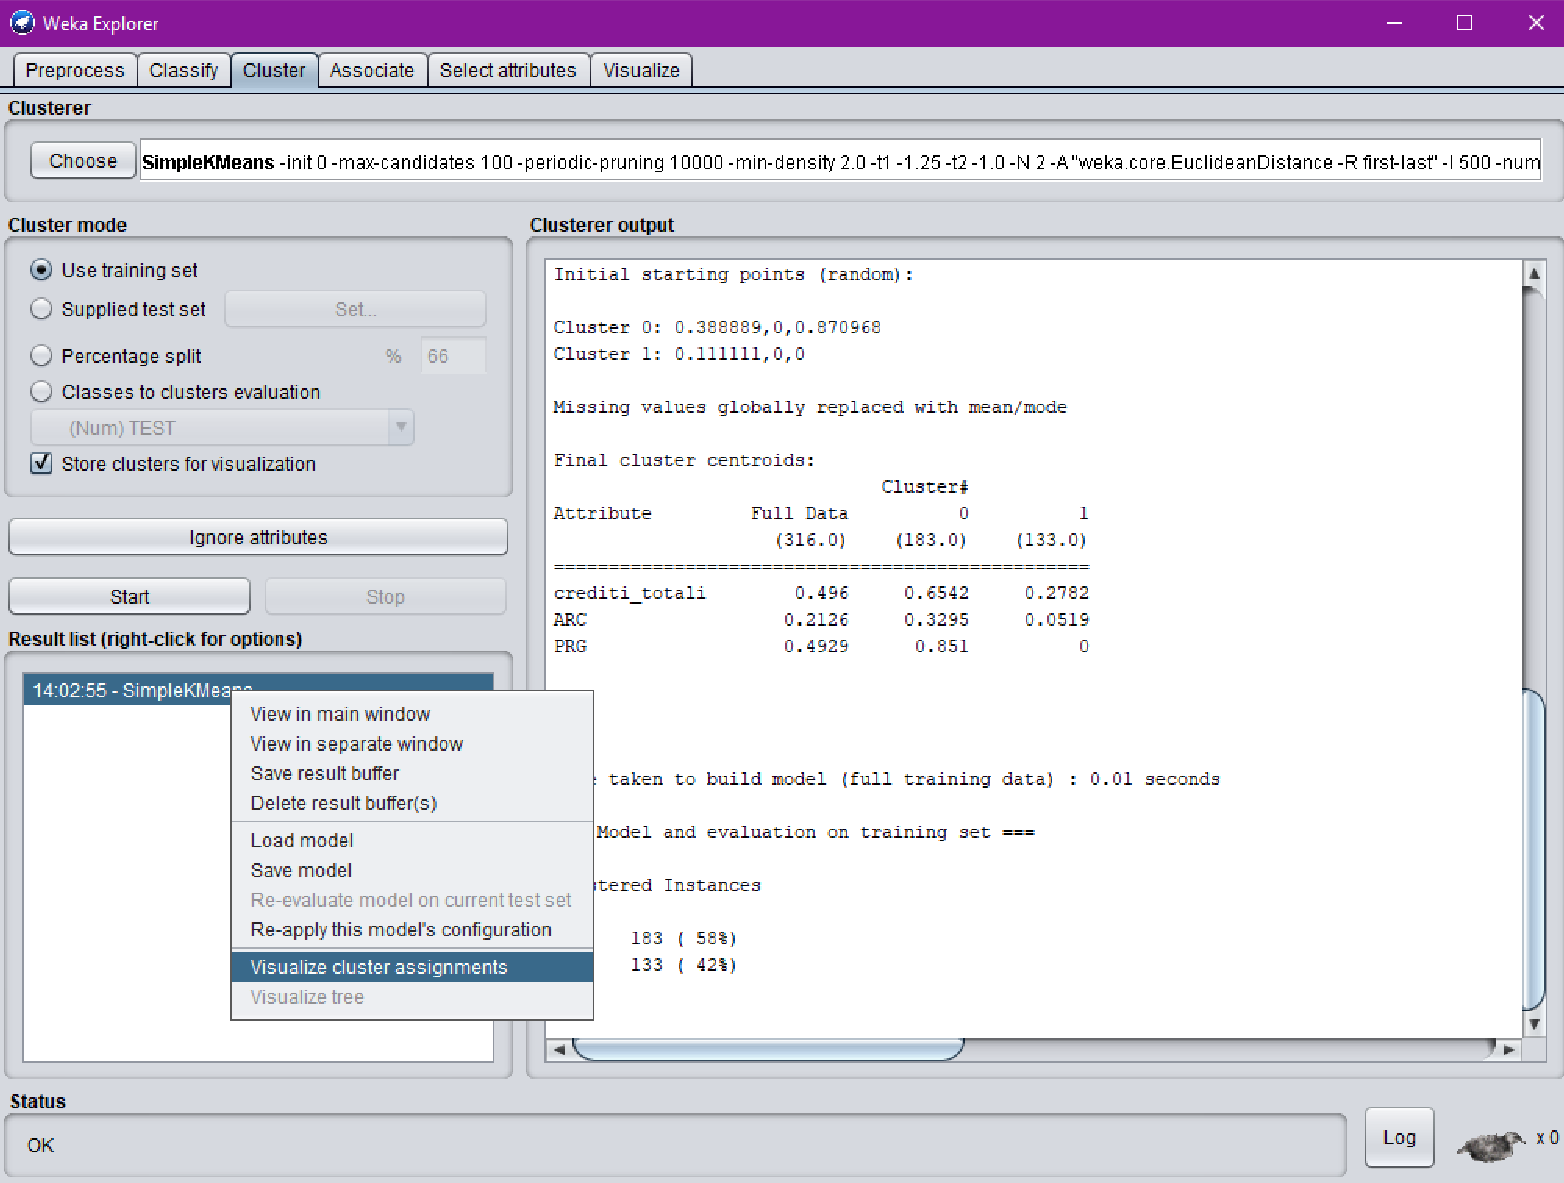
\includegraphics[width=\textwidth]{img/save-cluster-ass-1.pdf}
	\end{subfigure}
	\begin{subfigure}[b]{0.496\textwidth}
	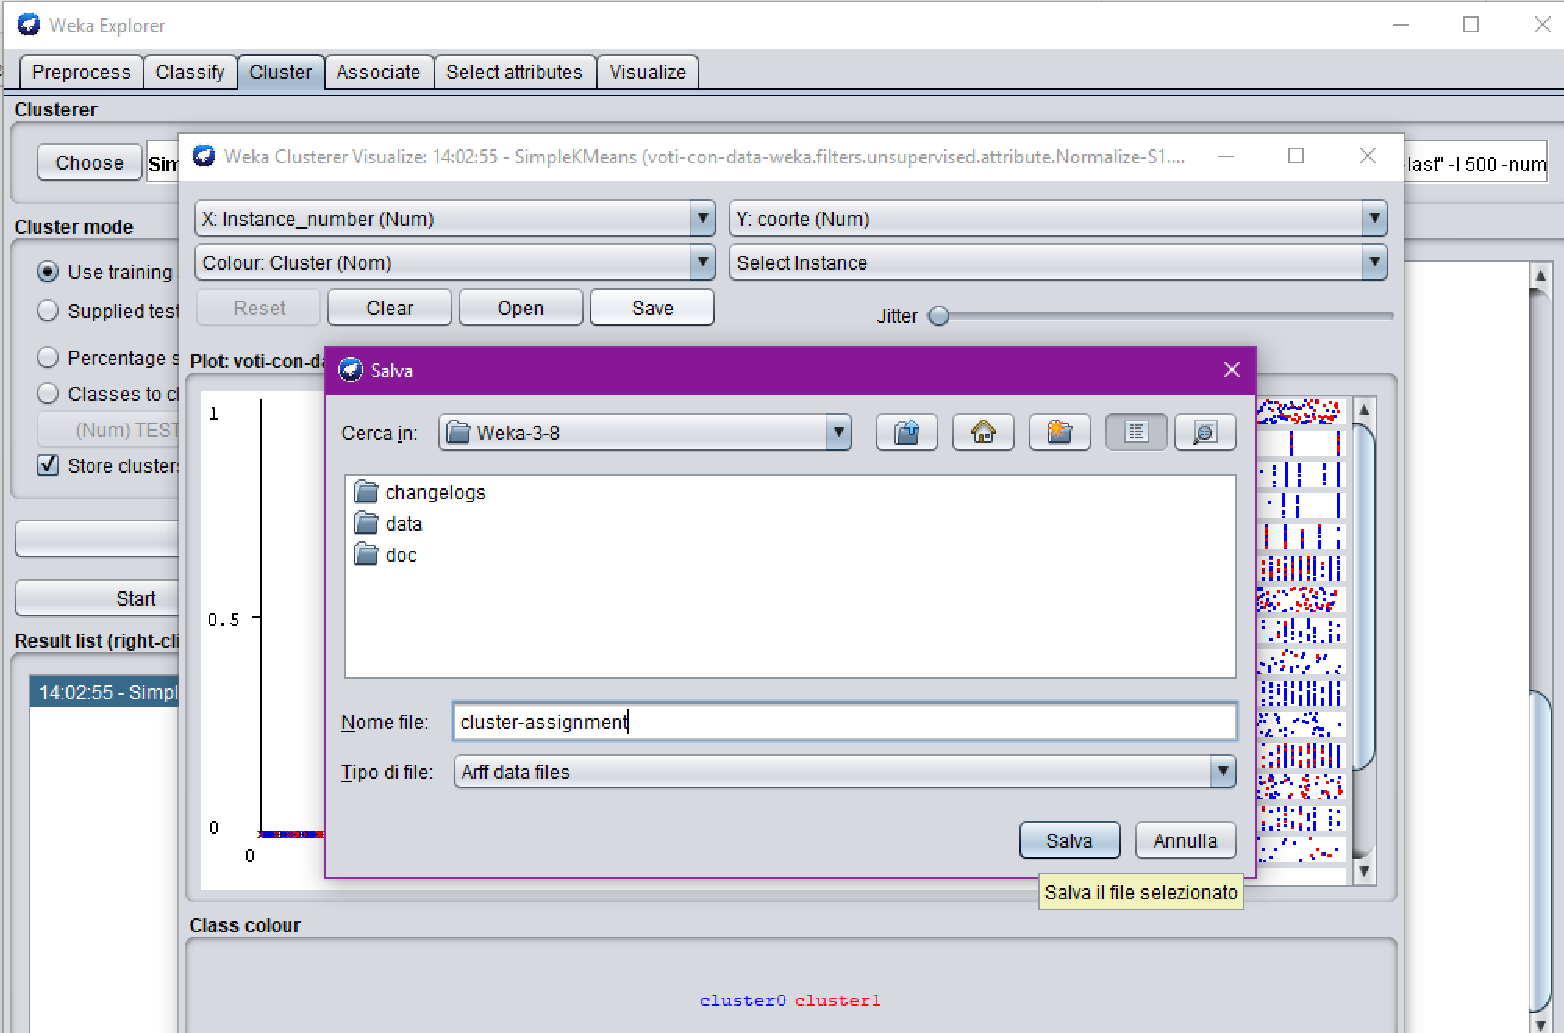
\includegraphics[width=\textwidth]{img/save-cluster-ass-2.pdf}
	\end{subfigure}

	\begin{subfigure}[b]{0.496\textwidth}
		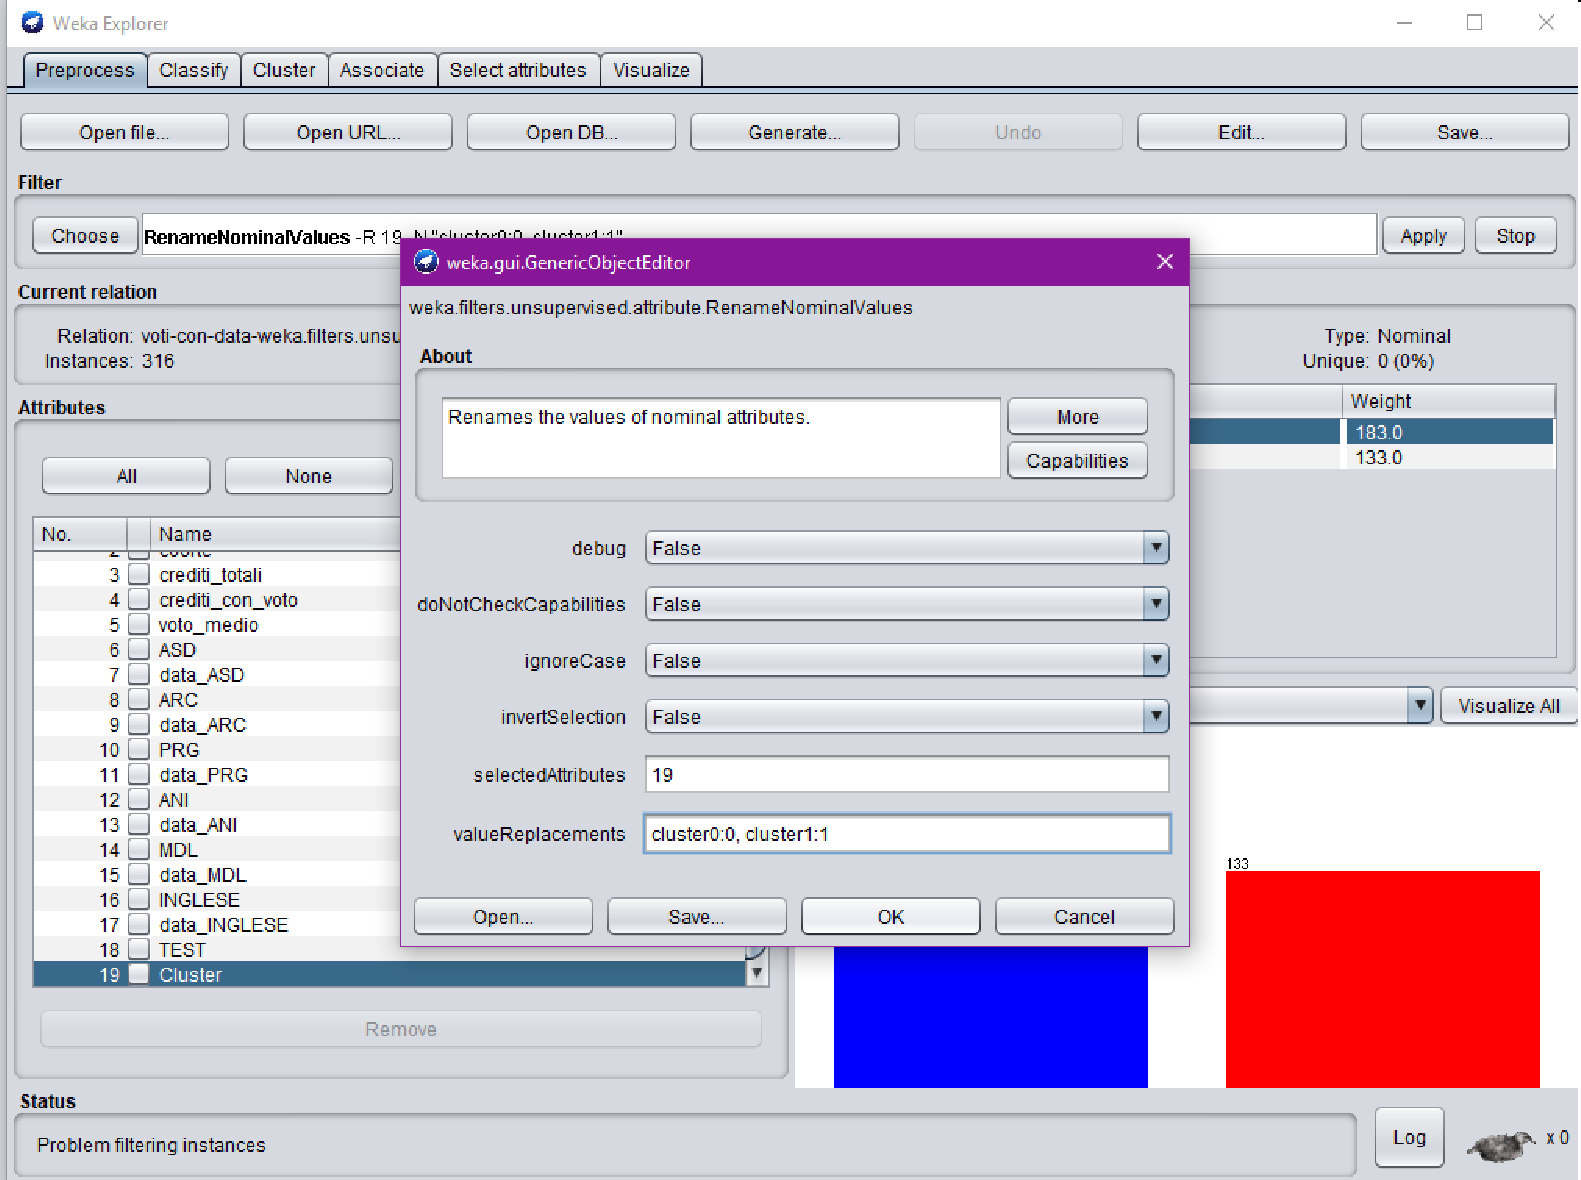
\includegraphics[width=\textwidth]{img/save-cluster-ass-3.pdf}
		\end{subfigure}
		\begin{subfigure}[b]{0.496\textwidth}
		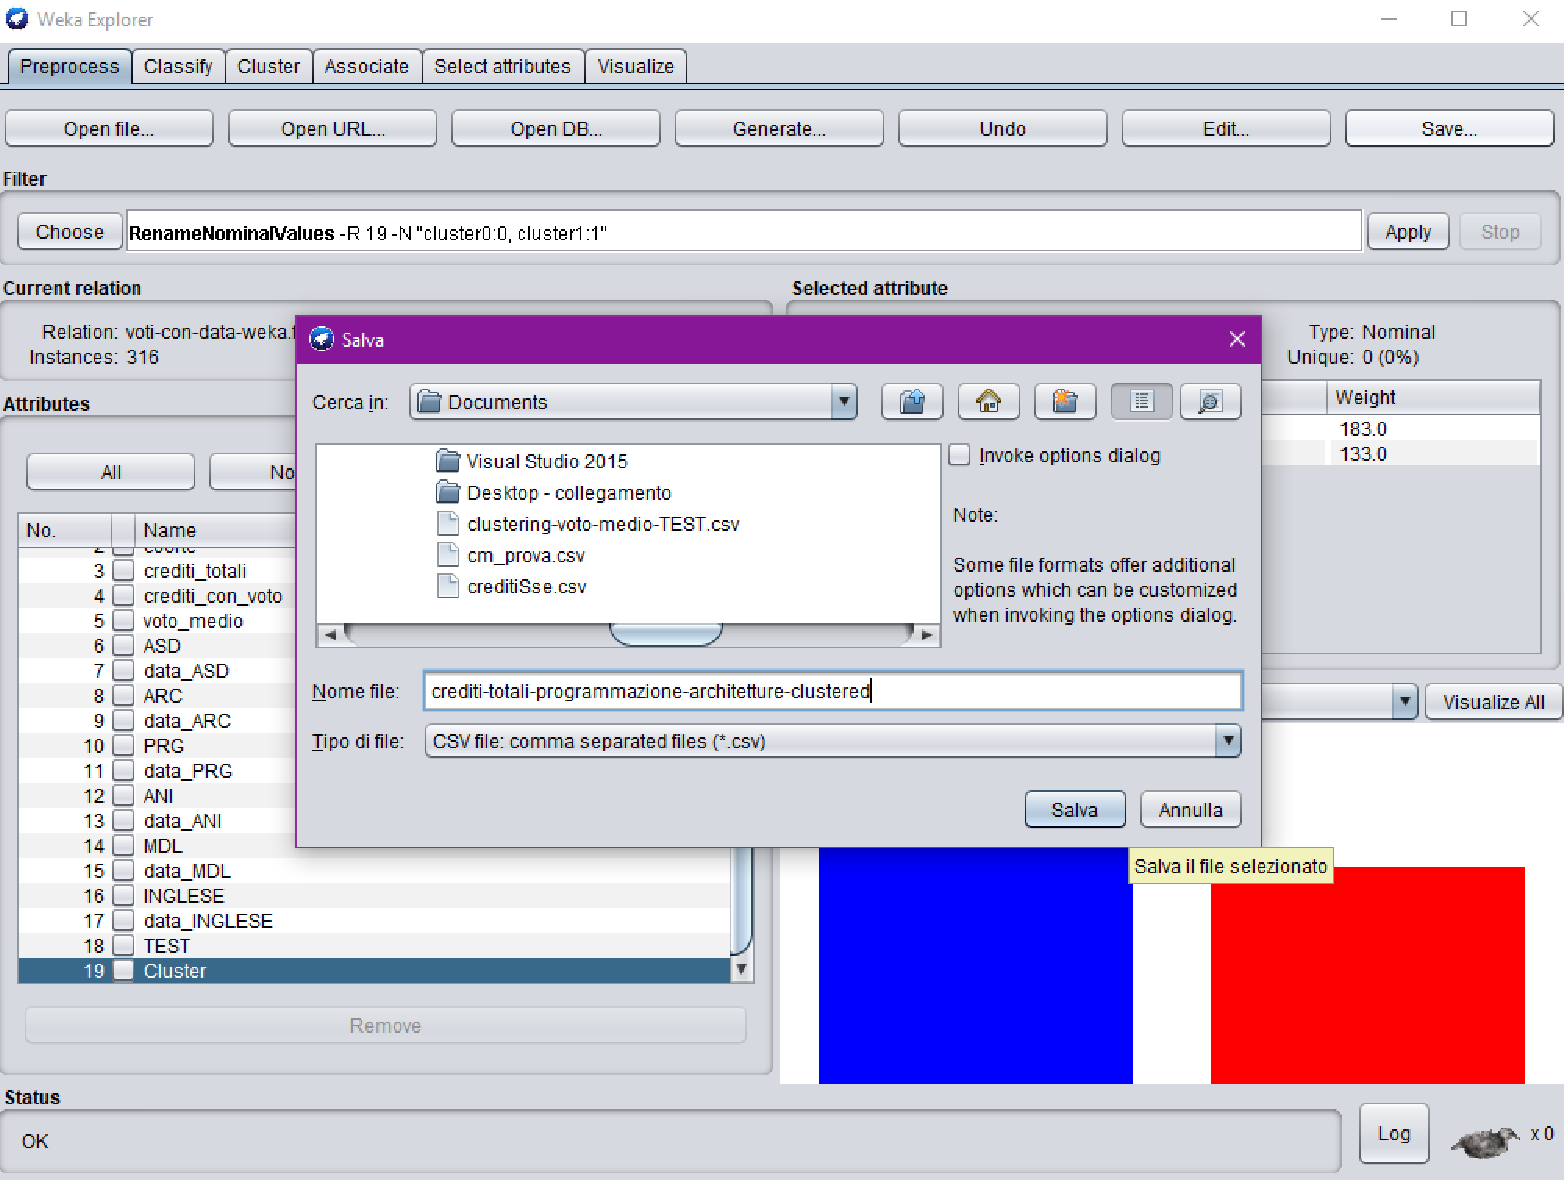
\includegraphics[width=\textwidth]{img/save-cluster-ass-4.pdf}
		\end{subfigure}
		\caption{creazione ed esportazione del dataset con indicazione del cluster di appartenenza in Weka.}
		\label{fig:add-cluster}
\end{figure}
\newpage
Nel Codice \ref{datacluster} viene mostrato come importare il dataset comprensivo degli attributi crediti totali, architetture, programmazione e cluster con R, mentre il Codice \ref{matrix-cor1} calcola la Matrice di incidenza dei cluster, la Matrice delle distanze per i punti e, infine, la correlazione tra le due matrici. 
Come si evince dal codice, per poter calcolare il valore della correlazione è stato necessario linearizzare preventivamente le due matrici utilizzando l'istru\-zione \texttt{as.vector} di \texttt{R}.

\lstset{%
   breaklines=true
}

\begin{lstlisting}[caption={Importazione degli attributi crediti totali, architetture, programmazione e cluster.}, label={datacluster}, captionpos=b, style = R]
library(readr)
crediti_totali_prg_arc_clustered <- read_csv("dmo/crediti_totali-prg-arc-clustered.csv", 
    col_types = cols(ANI = col_skip(), ASD = col_skip(), 
        INGLESE = col_skip(), Instance_number = col_skip(), 
        MDL = col_skip(), TEST = col_skip(), 
        coorte = col_skip(), crediti_con_voto = col_skip(), 
        data_ANI = col_skip(), data_ARC = col_skip(), 
        data_ASD = col_skip(), data_INGLESE = col_skip(), 
        data_MDL = col_skip(), data_PRG = col_skip(), 
        voto_medio = col_skip()))
View(crediti_totali_prg_arc_clustered)
\end{lstlisting}

\begin{lstlisting}[caption={Calcolo Matrice di incidenza dei cluster, delle distanze e correlazione tra le due matrici.}, label={matrix-cor1}, captionpos=b, style = R]
# Matrice di incidenza
matriceIncidenza <- function(data){
  nr = nrow(data)
  nc = ncol(data)
  C = matrix(nrow = nr, ncol = nr)
  for(i in 1:nr){
	for(j in 1:nr){
	  if(data[i,nc] == data[j,nc])
		C[i,j] = 1
	  else
		C[i,j] = 0
	}
  }
  return(C)
}

# matrice distanza
matriceDistanza <- function(data){
  return(as.matrix(dist(data[,1:(ncol(data)-1)],method = 'euclidean',diag = TRUE,upper = TRUE)))
}

calcoloCorrelazione <- function(data){
  MI <- matriceIncidenza(data)
  D <- matriceDistanza(data)
  mi = as.vector(t(MI))
  d = as.vector(t(D))
  
  return(cor(mi,d,method="pearson"))
}

calcoloCorrelazione(crediti_totali_prg_arc_clustered)
\end{lstlisting}	

\begin{lstlisting}[caption={Codice Java per il calcolo di SSE al variare di K}, label={javasse}, captionpos=b, style = java]
import weka.core.Instances;
import weka.core.converters.ConverterUtils.DataSource;
import weka.filters.Filter;
import weka.filters.unsupervised.attribute.Normalize;
import weka.clusterers.SimpleKMeans;
import weka.filters.unsupervised.attribute.Remove;

import java.io.FileWriter;
import java.io.IOException;
import java.util.ArrayList;

public class SseWeka {

	public static void main(String[] args) throws Exception {
		DataSource source = new DataSource("./voti-con-data.arff");
		Instances data = source.getDataSet();
		data.setClassIndex(-1);

		Normalize normalize = new Normalize();
		normalize.setInputFormat(data);
		Instances nData = Filter.useFilter(data, normalize);

		Remove remove = new Remove();
		// 0 coorte,1 crediti_totali,2 crediti_con_voto,3 voto_medio,4 ASD,5 data_ASD,6 ARC,7 data_ARC,
		// 8 PRG,9 data_PRG,10 ANI,11 data_ANI,12 MDL,13 data_MDL,14 INGLESE,15 data_INGLESE,16 TEST
		int[] attributeIndexesToRemove = {1,6,8};
		remove.setInvertSelection(true);
		remove.setAttributeIndicesArray(attributeIndexesToRemove);
		remove.setInputFormat(nData);
		Instances creditiArcPrg = Filter.useFilter(nData, remove);

		SimpleKMeans kMeans = new SimpleKMeans();
		kMeans.setPreserveInstancesOrder(true);

		int maxK = 50;
		int minK = 2;
		ArrayList<double[]> resultSet = new ArrayList<double[]>(maxK);
		double[] a;
		for (int i = minK; i < maxK; i++) {
			kMeans.setNumClusters(i);
			kMeans.buildClusterer(creditiArcPrg);
			a = new double[2];
			a[0] = i; a[1] = kMeans.getSquaredError();
			resultSet.add(a);
		}
		for (int i = 0; i < maxK - minK; i++) {
			System.out.println(resultSet.get(i)[1]);
		}

		try {
			FileWriter writer = new FileWriter("creditiArcSse.txt", false);

			for (int i = minK; i < maxK; i++)
				writer.write(i + "," + resultSet.get(i - minK)[1] + "\r\n");
			writer.close();
		} catch (IOException e) {
			e.printStackTrace();
		}

	}
}		
\end{lstlisting}
Il valore di correlazione ottenuto in questo caso è pari a $-0.687$.
Ripetendo il clustering per gli stessi attributi con $k=3$ e $k=18$ si ottiene, 
rispetti\-vamente un valore della correlazione tra le due matrici di $-0.854$ e $-0.489$. 

Diversamente da quanto atteso, il valore calcolato per $k_{opt}$ non presenta un valore di correlazione 
inferiore rispetto agli altri due clustering, 
bensì risulta essere il valore peggiore tra quelli verificati con il metodo della correlazione. 
In Figura \ref{fig:k-sse2} e Figura \ref{fig:k-sse3} sono riportati i grafici dell'andamen\-to 
del $SSE$ in funzione di $k$ per, rispettivamente, 
l'analisi condotta sui voti conseguiti dagli studenti nelle cinque materie del primo anno e l'analisi relativa al voto medio e al risultato del test. 
Scegliendo quindi nuovamen\-te $\varepsilon=0.01$ i valori di $k_{opt}$ sono, rispettivamente $36$ e $43$. 

\begin{table}[H]
\centering
\begin{tabular}{@{}l|l|l@{}}
\hline
\textbf{Attributi analizzati}   							& \textbf{k} & \textbf{Correlazione} \\ \hline
                                							& 2          & -0.687                \\ \cline{2-3} 
crediti totali, ARC, PRG        							& 3          & -0.854                \\ \cline{2-3} 
                                							& 18         & -0.489                \\ \hline
                                							& 2          & -0.520                \\ \cline{2-3} 
ARC, ASD, PRG, MDL,	AN1	\hspace{3em}									& 3          & -0.618                \\ \cline{2-3} 
                                							& 36         & -0.424                \\ \hline
                                							& 2          & -0.476                \\ \cline{2-3} 
voto medio, test                							& 3          & -0.465                \\ \cline{2-3} 
                                							& 43         & -0.273                \\ \hline
\end{tabular}
\caption{Valori correlazione tra la Matrice di incidenza dei cluster e la matrice delle distanze in funzione di $k$.}
\label{tab:corr2}
\end{table}

In Tabella \ref{tab:corr2} sono riportate sinteticamente le correlazioni ottenute per ciascuna delle tre analisi condotte in funzione dei diversi valori di $k$ scelti. Come è possibile notare consultando la Tabella \ref{tab:corr}, anche nella seconda e terza analisi il valore di $k$ scelto consultando il grafico $k-SSE$ risulta essere il peggiore contrariamente alle aspettative.

\begin{figure}[H]
	\centering
	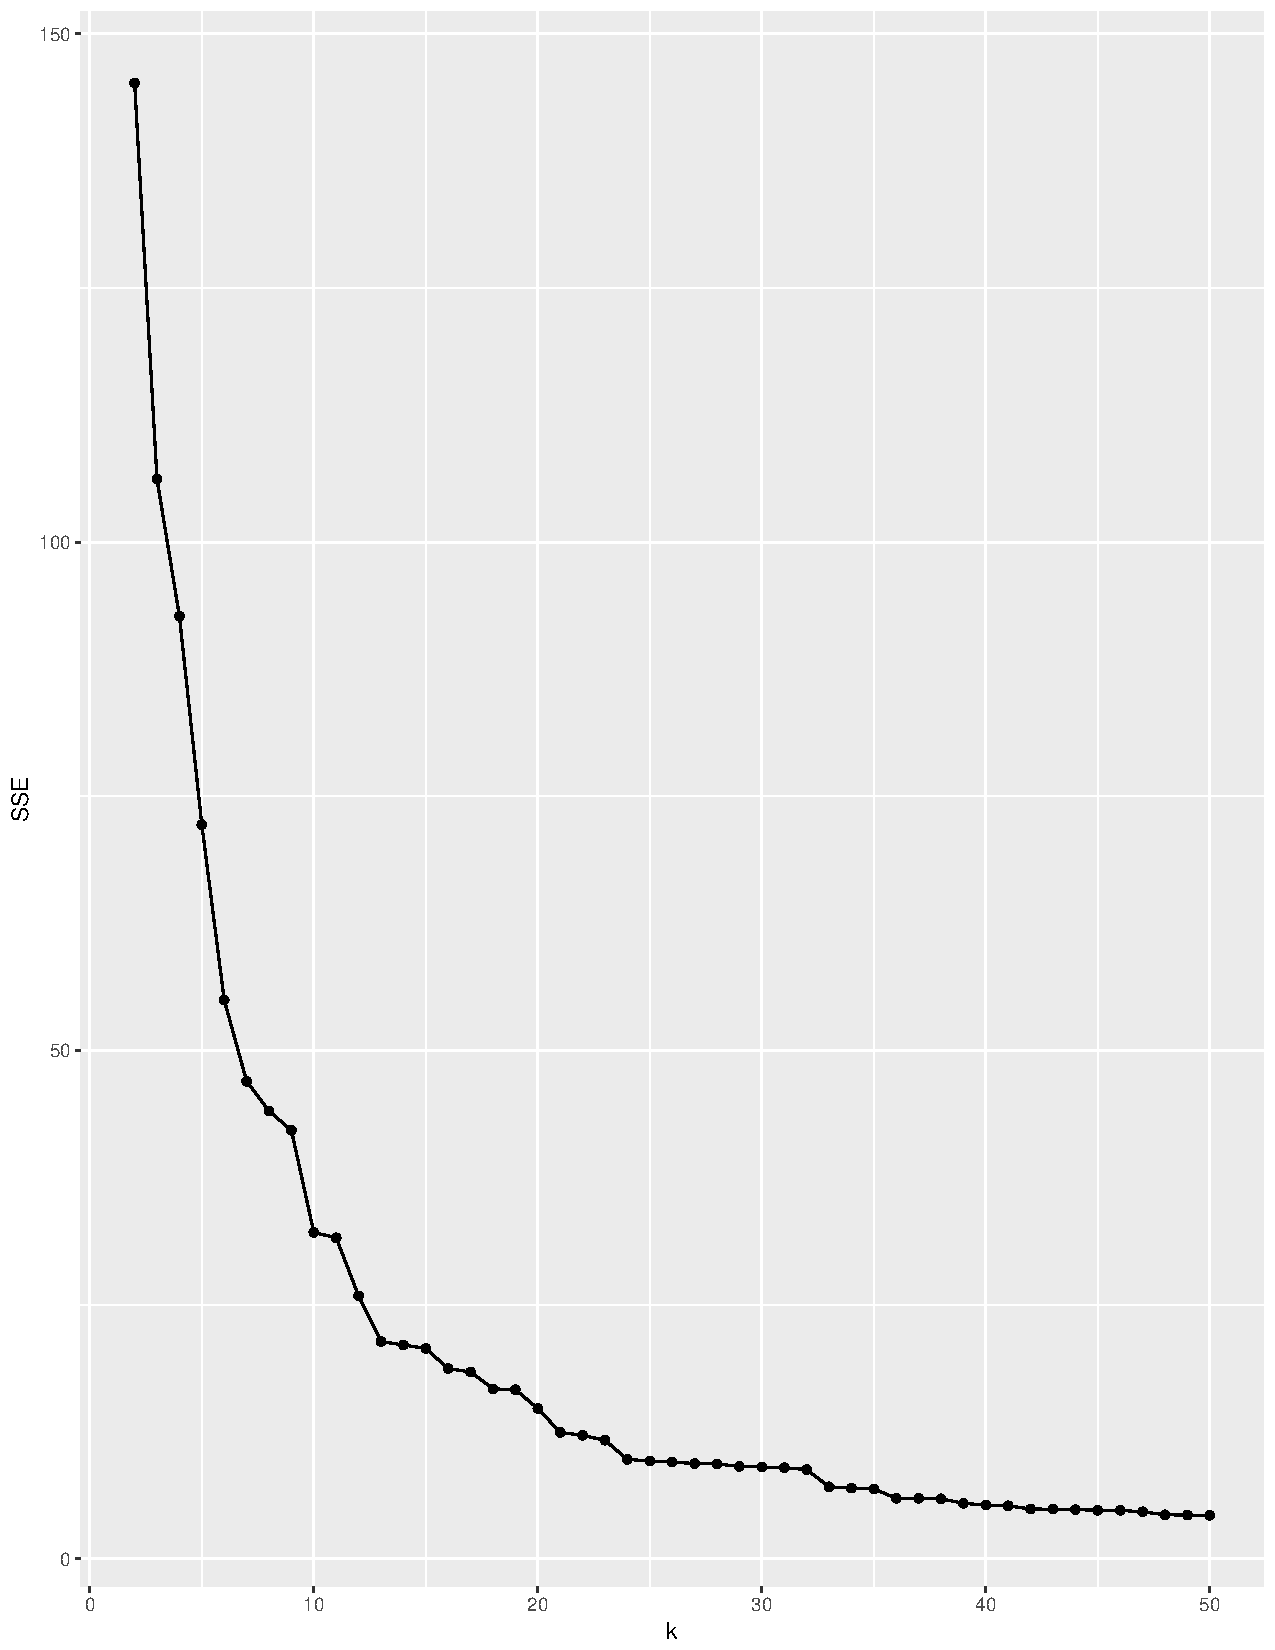
\includegraphics[width=\textwidth, height=12cm,keepaspectratio]{img/k-sse-asd-arc-prg-an1-mdl.pdf}
	\caption{Andamento del valore del $SSE$ in funzione del valore di $k$ per i voti di architetture, programmazione, algoritmi e strutture dati, analisi matematica 1 e matematica discreta e logica.}
	\label{fig:k-sse2}
\end{figure}

\begin{figure}[H]
	\centering
	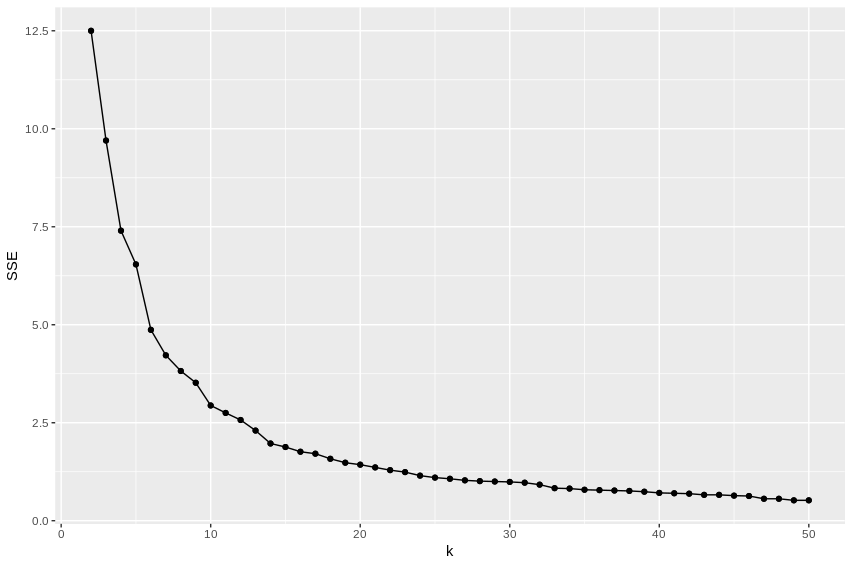
\includegraphics[width=\textwidth, height=12cm,keepaspectratio]{img/k-sse-voto_medio-test.png}
	\caption{Andamento del valore del $SSE$ in funzione del valore di $k$ per il voto medio e il voto del test.}
	\label{fig:k-sse3}
\end{figure}

Una possibile spiegazione di questo fenomeno è la seguente: aumen\-tando notevolmente il numero di cluster $k$ è probabile che record vicini vengano posti in cluster differenti soprattutto se i centroidi di quest'ultimi sono anch'essi molto vicini. 
Quando si verifica questa circostanza il valore di incidenza nella matrice dei cluster è $0$ anche se la corrispettiva distanza tra due record è molto piccola andando così a ridurre il modulo della correlazione (negativa) che esiste tra i valori delle due matrici. 
È possibile calcolare il valore di correlazione (e quindi valutare la bontà del cluste\-ring) tra matrice di incidenza dei cluster e matrice delle distanze anche nel clustering calcolato dall'algoritmo DBSCAN. 
Tale metodo è stato utilizza\-to nell'analisi relativa ai voti conseguiti dagli studenti nelle cinque materie del primo anno. 
Tuttavia, in questa circostanza è necessario provvedere all'eliminazione dal dataset dei record marcati come rumore da DBSCAN e quindi sarà necessario tener conto non solo del valore di correlazione ottenuto, ma considerare anche quanti dati vengono esclusi eseguendo l'algoritmo con certi parametri. 

La Figura \ref{fig:remove-noise} mostra con che valori inizializzare i parametri del filtro di Weka \texttt{RemoveWithValues} al fine di eliminare dal dataset i record marcati come rumore. La Tabella \ref{tab:corr-noise-dbscan} riporta sinteticamente i valori di correlazione e numero di record etichettati come rumore ottenuti per ogni esecuzione dell'algoritmo DBSCAN con i diversi parametri utilizzati. Come si evince dalla Tabella \ref{tab:corr-noise-dbscan} l'esecuzione ottimale del DBSCAN è ottenuta con \texttt{MinPts = 20} e \texttt{eps=0.4}. Tale risultato ha tuttavia un prezzo: i record etichettati in questo caso sono $89$ ossia più del doppio rispetto alle altre due esecuzioni prese in considerazione. Inoltre, considerando la Tabella \ref{tab:corr} è possibile concludere che, l'algoritmo DBSCAN determina dei clustering migliori rispetto a K-means per l'analisi relativa ai voti conseguiti dagli studenti.

\begin{figure}[H]
\centering
	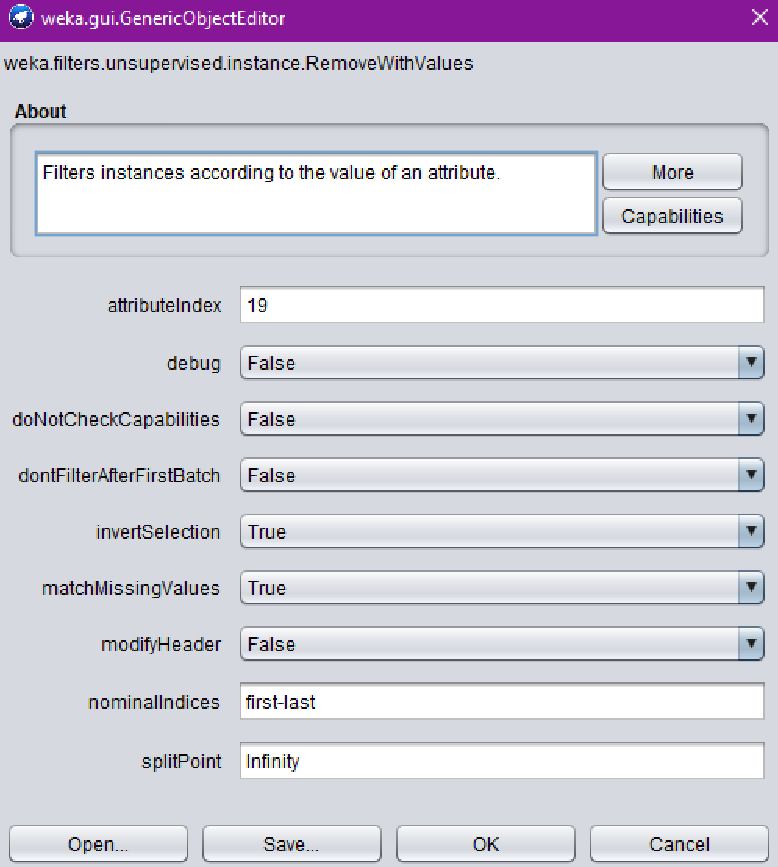
\includegraphics[width=0.7\textwidth]{img/filter-for-remove-noise.pdf}
	\caption{Valori da impostare nei parametri del filtro \texttt{RemoveWithValues} di Weka.}
	\label{fig:remove-noise}
\end{figure}

\begin{table}[H]
\centering
\begin{tabular}{@{}lll@{}}
\toprule	
\texttt{MinPts}, \texttt{eps} & Correlazione & Rumore \\ \hline
$6$,$0.5$       & $-0.725$  & $38$     \\ 
$10$,$0.4$      & $-0.728$  & $44$     \\ 
$20$,$0.4$      & $-0.758$  & $89$     \\ \bottomrule
\end{tabular}
\caption{Valori riepilogativi di correlazione e rumore per DBSCAN}
\label{tab:corr-noise-dbscan}
\end{table}

Fino a questo momento è stata analizzata la bontà del clustering fornito da DBSCAN con i parametri scelti in maniera arbitraria basandosi sull'in\-tuito e la conoscenza del problema. 
In maniera del tutto analoga a quanto fatto per l'algoritmo di K-means è possibile utilizzare una procedura di model selection che cerchi di stabilire il modello (e quindi i parametri) ottimale. Nel caso di DBSCAN la procedura che verrà utilizzata cerca di determinare il valore ottimale di \texttt{eps} fissando il valore di \texttt{MinPts} basandosi sull'idea che i $k$-esimi vicini dei punti contenuti in un cluster sono più o meno posti alla stessa distanza mentre i punti etichettati come rumore hanno il $k$-esimo vicino a una distanza maggiore. 
Basandosi su questo fatto è possibile determinare un grafico che sulle ascisse contiene gli indici dei record ordinati in modo non decrescente rispetto alla distanza dal loro $k$-esimo record più vicino e sulle ordinate mostra il valore di tale distanza. 
Come valore di \texttt{eps} è quindi possibile scegliere la prima distanza che è "sufficientemente" maggiore dalle precedenti. 

Nel Codice \ref{rknn} è mostrata la funzione in R che determina il grafico in questione e la riga di codice per calcolare tale grafico nel caso in cui \texttt{MinPts=6}. 
In Figura \ref{fig:eps-minpts6} è riportato il grafico dei valori delle distanze dei punti dal $k$-6-esimo più vicino. 
Come si può notare dalla figura, il valore ottimale indicato per \texttt{eps} è maggiore di $0.4$ e minore di $0.6$ e quindi il valore di \texttt{eps} risulta essere una buona scelta. 
La Figura \ref{fig:eps-minpts10} e la Figura \ref{fig:eps-minpts20} riportano, rispettivamente, le distanze dei punti dal loro $k$-10-esimo più vicino e dal loro $k$-20-esimo più vicino. 
Nel primo caso, il valore \texttt{eps} scelto inizialmen\-te è confermato da quanto riportato dalla Figura \ref{fig:eps-minpts10}, mentre la Figura \ref{fig:eps-minpts20} suggerisce di scegliere un valore di \texttt{eps} maggiore di $0.5$ per l'esecuzione del DBSCAN con \texttt{MinPts=20}. 
Tuttavia, l'esecuzione di DBSCAN con la combinazione di tali parametri non ha prodotto risultati significativi.

\begin{minipage}{\linewidth}
\begin{lstlisting}[caption={Codice R per il calcolo del grafico della k-esima distanza da ogni punto del dataset.}, label={rknn}, captionpos=b, style = R]
kDBScan <- function(data,k){
  library(ggplot2)
  D = as.matrix(dist(data[,1:ncol(data)-1],method = 'euclidean',diag = TRUE,upper = TRUE))
  D_1 = D
  for(i in 1:nrow(data)){
    D_1[i,] = sort(D[i,])
  }
  p = 1:nrow(data)
  dist = sort(D_1[, k])
  data = data.frame(p,dist)
  ggplot(data, aes(x=p, y=dist)) +geom_point(shape=1) +  geom_line() + geom_point(color = 'black')
}

kDBScan(crediti_totali_prg_arc_clustered, 6)
\end{lstlisting}
\end{minipage}
\begin{figure}[H]
\centering
	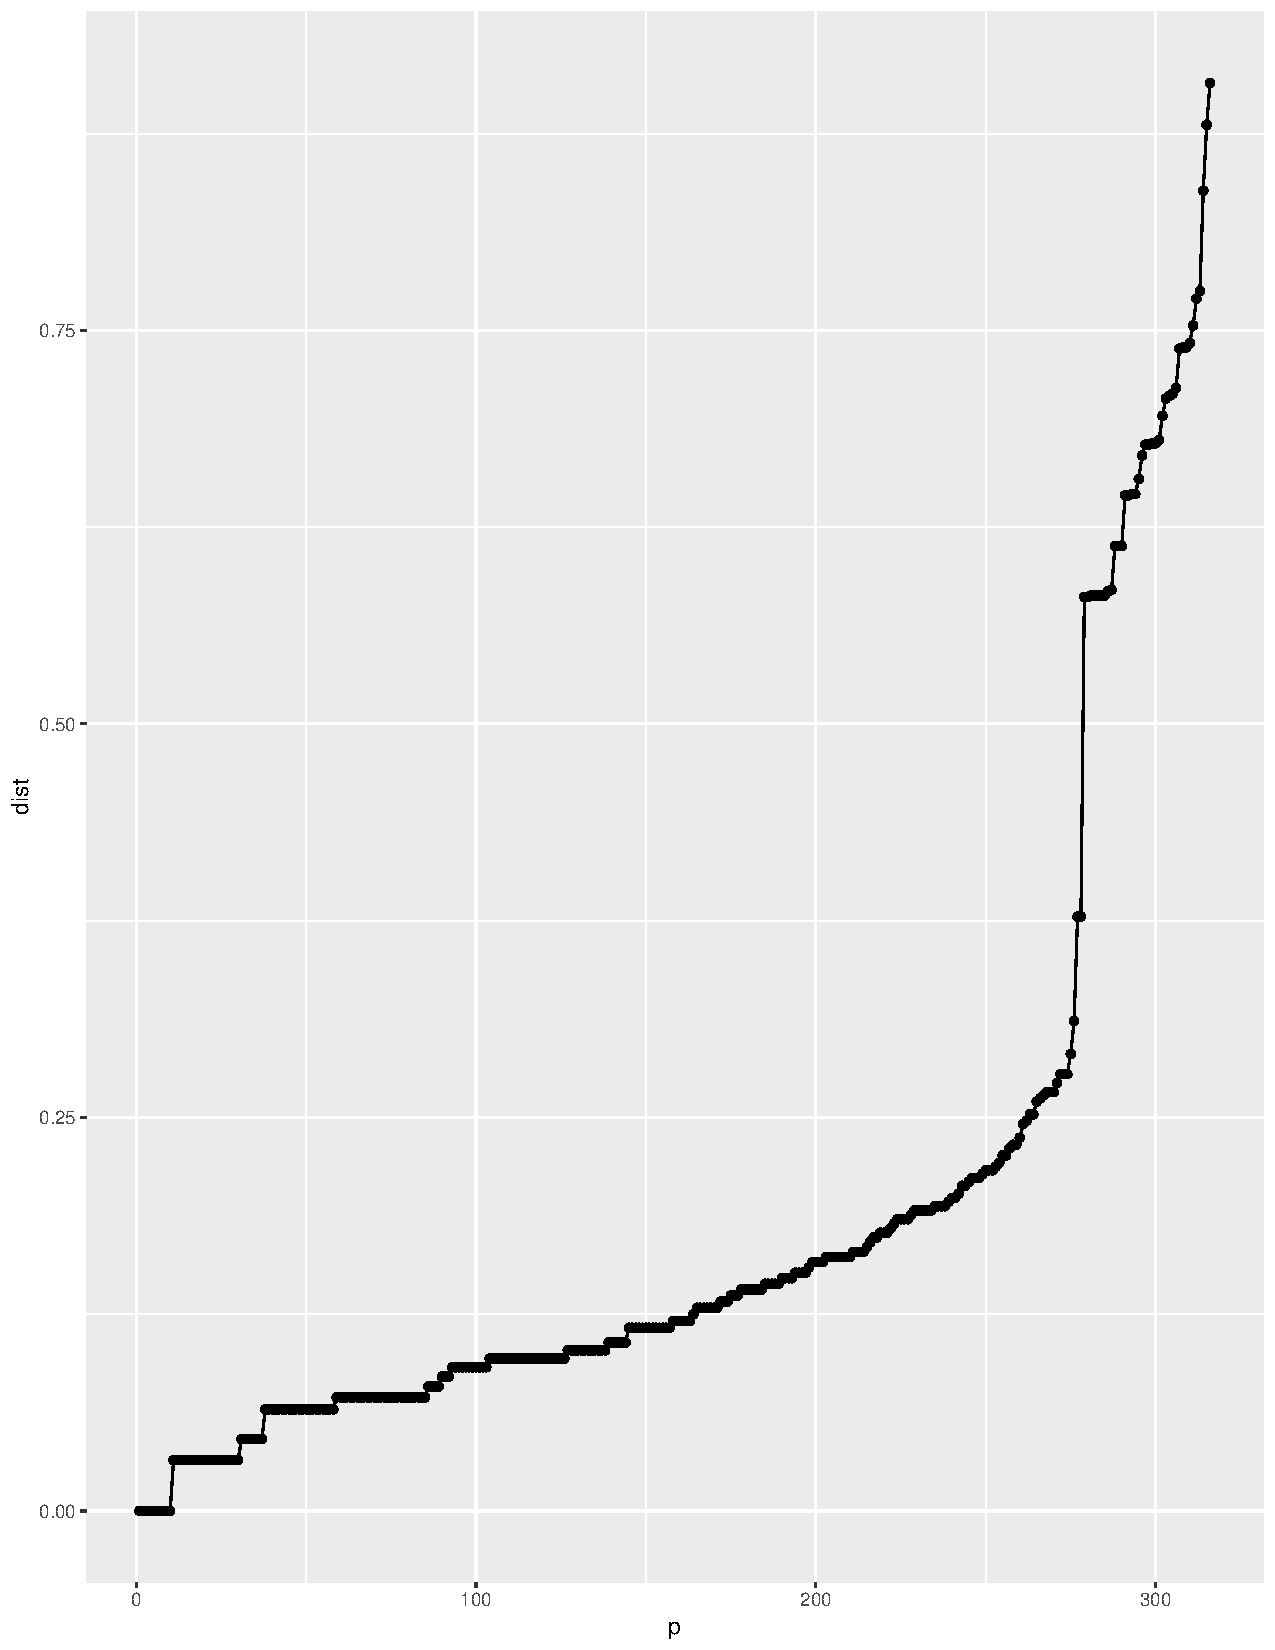
\includegraphics[width=\textwidth]{img/eps-minpts6.pdf}
	\caption{Distanze dei punti dal $k=6$-esimo più vicino.}
	\label{fig:eps-minpts6}
\end{figure}

\begin{figure}[H]
\centering
	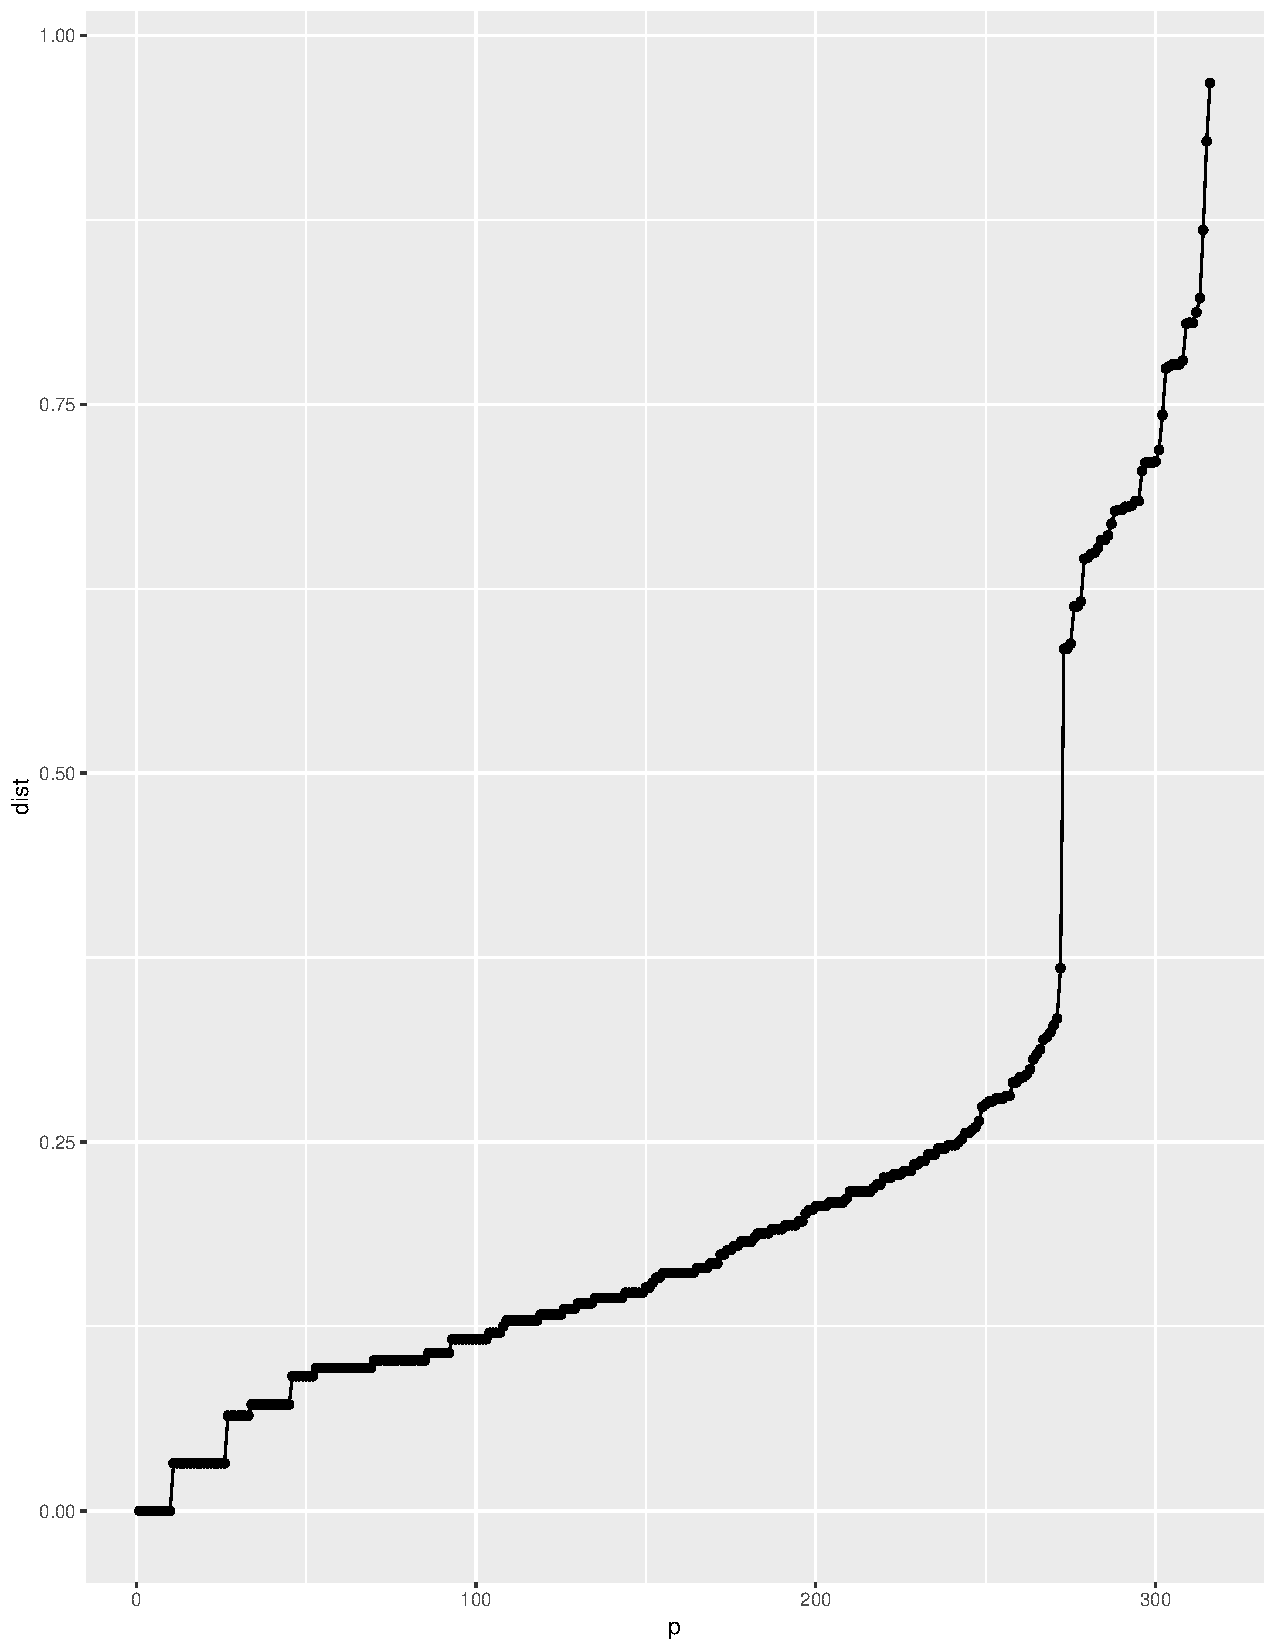
\includegraphics[width=\textwidth]{img/eps-minpts10.pdf}
	\caption{Distanze dei punti dal $k=10$-esimo più vicino.}
	\label{fig:eps-minpts10}
\end{figure}

\begin{figure}[H]
\centering
	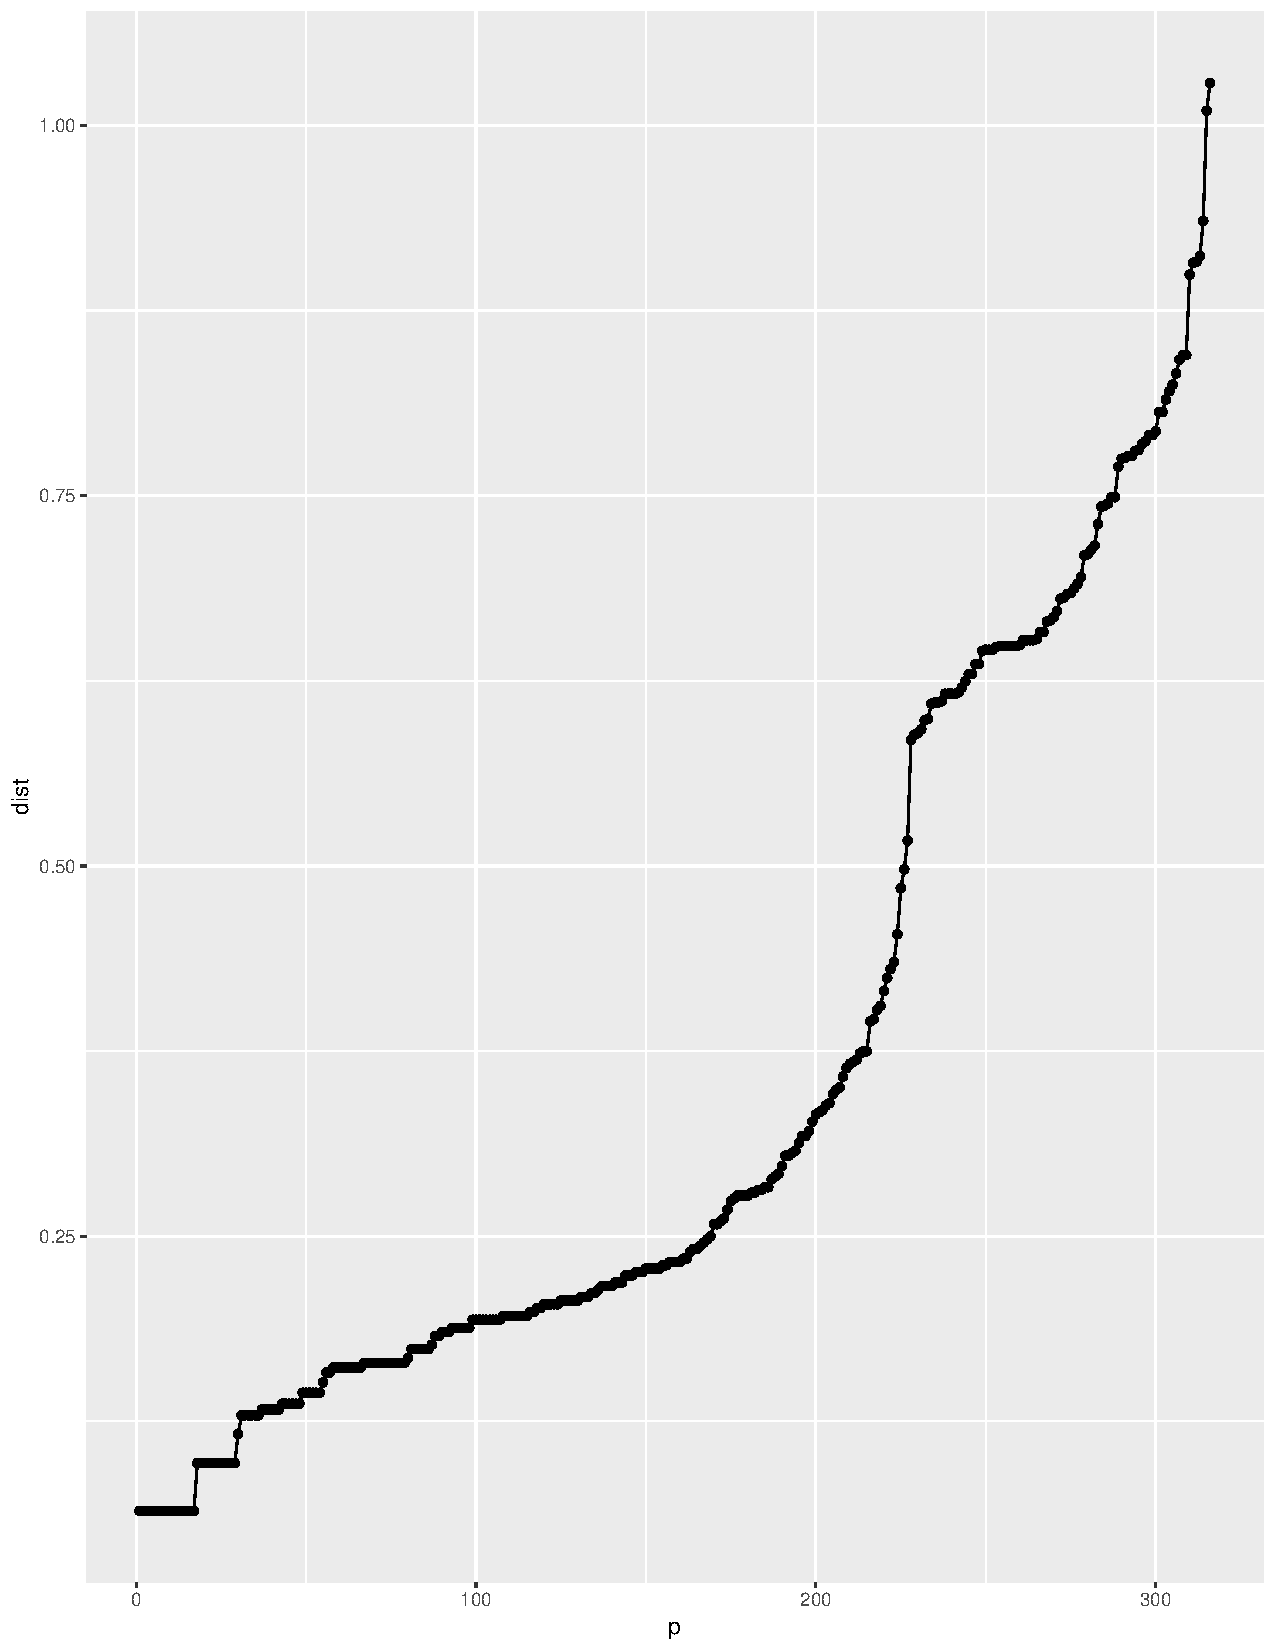
\includegraphics[width=\textwidth]{img/eps-minpts20.pdf}
	\caption{Distanze dei punti dal $k=20$-esimo più vicino.}
	\label{fig:eps-minpts20}
\end{figure}

In Tabella \ref{tab:mod-opt} sono riportati i modelli ottimali determinati per i tre diver\-si aspetti del dataset che sono stati analizzati. 
Tali modelli sono stati scelti basandosi esclusivamente sul valore della correlazione tra la matrice di incidenza dei cluster e la matrice delle distanze e quindi nel caso di DBSCAN non viene tenuto conto della maggior perdita di dati che vengono etichet\-tati come rumore nel modello ottimale riportato in Tabella \ref{fig:eps-minpts20}. 
In ogni caso, tenendo conto anche di questo aspetto, DBSCAN si è rilevato essere un algoritmo affidabile per l'analisi su cui è stato eseguito e anche l'esecu\-zione con gli altri parametri ha portato a risultati paragonabili a quelli del modello ottimale e decisamente migliori di quelli ottenuti con il K-means.

\begin{table}[H]
\begin{adjustbox}{max width=\textwidth}
\begin{tabular}{@{}llll@{}}
\toprule
Attributi analizzati     & Algoritmo Migliore & Parametri ottimali & Correlazione \\ \midrule
crediti totali, ARC, PRG & K-means            & $k=3$                & $-0.854$       \\
ARC, ASD, PRG, MDL, AN1  & DBSCAN             & \texttt{MinPts=20},\texttt{eps=0.4}  & $-0.758$ \\
voto medio, test         & K-means            & $k=2$                & $-0.476$       \\ \bottomrule
\end{tabular}
\end{adjustbox}
\caption{Modelli ottimali.}
\label{tab:mod-opt}
\end{table}

\newpage

\section{Conclusioni}
In riferimento ai risultati ottenuti con il K-means è possibile trarre le seguenti conclusioni riguardo
le carriere degli studenti:
\begin{itemize}
\item l'esame di Architetture degli Elaboratori risulta essere l'esame più difficile per gli studenti del primo anno,
  infatti la maggioranza non riesce a sostenerlo nel corso della sessione estiva. Tuttavia, general\-mente gli studenti 
  che sostengono con profitto tale esame riescono a sostenere con un buon voto anche gli altri; 
\item la maggior parte degli studenti che ottengono un buon punteggio al test d'ingresso mantengono una buona media
  mentre quelli che hanno ottenuto un punteggio più basso hanno anche una media più bassa. Tuttavia è presente
  un significativo gruppo di studenti che pur avendo ottenuto un buon punteggio al test di ingresso non rie\-scono
  ad avere una media altrettanto buona;
\item La maggior parte degli studenti riesce a sostenere nel corso della sessione estiva gli esami di Algoritmi e 
  Strutture Dati, Analisi I e in alcuni casi l'esame di Programmazione con risultati altalenanti. Mentre 
  generalmente gli esami di Architetture degli Elaborati e Ma\-tematica Discreta e Logica non vengono sostenuti
  dagli studenti al termine del loro primo anno.
\end{itemize}
Inoltre, in ciascuna delle analisi eseguite risultavano esserci almeno 3 gruppi di studenti che presentavano 
caratteristiche significativamente differenti.

La tecnica del DBSCAN è risultata essere efficace e ha consentito di determinare dei clustering migliori rispetto a quelli determinati dal K-means nell'analisi dei voti degli studenti. 
Diversamente dai clustering ottimali determinati dal K-means, i clustering del DBSCAN presentano un alto numero di cluster diversi ed è quindi difficile (e inconcludente) descrivere il profilo dello studente medio appartente a ciascuno gruppo. 
Tuttavia, è necessario tenere presente che i clustering determinati con questa tecnica etichettano una buona parte dei dati totali come rumore (quasi un terzo nel clustering ottimale) e quindi l'analisi viene condotta necessaria\-mente su un sottoinsieme del dataset. 

Infine, per quanto riguarda il clustering gerarchico, è stato scelto di condurre delle analisi sulla proiezione del dataset relativa all'anno di im\-matricolazione del 2010. 
Tale scelta è motivata dal fatto che gli studenti imma\-tricolati nei diversi anni non presentano caratteristiche (voti ai test, agli esami, crediti totali, etc.) significativamente differenti e dal fatto che i dendogrammi dell'intero dataset risultavano incomprensibili. 
In ogni caso, l'analisi condotta con tali tecniche è limitata poiché si è scelto di valutare il numero di cluster con le tecniche presentate nel capitolo \ref{cap:val-clust} e inoltre i relativi clustering non potevano essere valutati con il metodo della correlazione utilizzato nel capitolo \ref{cap:val-clust} per K-means e DBSCAN.
\newpage 

\listoffigures
 
\newpage

% \thispagestyle{empty}\clearpage\mbox{}\clearpage

\listoftables

\newpage

% \thispagestyle{empty}\clearpage\mbox{}\clearpage

\end{document}